\documentclass{plantilla}

\hypersetup{hidelinks}

\usepackage{xspace}

% ----------------------------------------------------------------------------

\title{Resumen Final} 
\subtitle{Bases de datos}
\author{(basado en resúmenes de CubaWiki, diapositivas y apuntes del 2do cuatrimestre de 2019, 
\\actualizado en 2022 por otro estudiante, Leandro N. Borgnia 
\\(este resumen no es mío pero me pareció muy completo y bien sintetizado y quería mejorarlo.))}
\date{6 de marzo de 2020}
%\updatemetadata 

% ----------------------------------------------------------------------------

\newenvironment{SQL}{
    \begin{center}
    \ttfamily}
    {\end{center}}

% ===========================================================

\begin{document}

\maketitle

% ===========================================================

\section*{Introducción}



\subsection*{Definiciones}
\begin{itemize}
    \item \textbf{Base de datos:} Es un conjunto de datos relacionados con un \textbf{significado inherente}. Esto hace que no consideremos a un conjunto de datos aleatorios como una, ya que se diseña y construye con un propósito específico. \\
    Surgieron en la década del '70 debido a las crecientes necesidades de almacenar y acceder a mayores cantidades de datos de forma eficiente. Suelen estar manejadas por un \textbf{DBMS} (Database Management System).
    \item \textbf{Dato:} Es un hecho conocido que puede ser registrado y tiene un significado implícito. Suele ser más volatil que la estructura en que está definido.
    \item \textbf{DML (Data Manipulation Language):} Es el usado en los DBMS para modificar las instancias: obtener, agregar, cambiar, etc. Algunas de sus funciones en SQL son SELECT, INSERT, DELETE.
    \item \textbf{DDL (Data Definition Language):} Se usa en los DBMS para alterar el esquema de la base: crear, agregar atributo, renombrar. Algunas de sus funciones en SQL son CREATE, ALTER, DROP, RENAME.
\end{itemize}

\subsection*{DBMS}
Es la herramienta que utiliza cada aplicación para manejar grandes cantidades de datos de manera eficiente. Suele ser configurada por los \textbf{administradores de bases de datos}.
Entre sus funciones tenemos:
\begin{enumerate}
    \item Permitirle a los usuarios crear nuevas bases de datos y especificar sus esquemas.
    \item Perimitirle a los usuarios realizar consultas a los datos y modificarlos.
    \item Almacenar grandes cantidades de datos por un período largo de tiempo para perimitir consultas y modificaciones eficientes.
    \item Garantizar la durabilidad de los datos al tener un sistema de recuperación en caso de fallas, errores o mal uso intencional. Este también se encarga de las copias de seguridad.
    \item Controlar el acceso concurrente a los datos por parte de los usuarios, de manera de evitar interacciones inesperadas y garantizar que las acciones realizadas sean seguras y completas.
\end{enumerate}
Otros componentes de la DBMS incluyen:
\begin{itemize}
    \item \textbf{Recovery Manager:} Encargado de restaurar la base de datos a un estado consistente en caso de haber una falla. Para hacer eso hace uso del \textbf{log}, un archivo que lleva un registro de las acciones efectuadas a la DB.
    \item \textbf{Optimizador de consultas:} Encargado de armar un plan de ejecución eficiente en base a una consulta, basándose en la información del \textbf{system catalog}.
\end{itemize}

\subsection*{System catalog}
Es el lugar de un \textbf{RDBMS} (Relational DBMS) en que se guardan los metadatos del esquema. Estos comprenden:
\begin{itemize}
    \item Información sobre tablas y columnas. Esto incluye datos estadísticos como el tamaño de los archivos y el factor de bloqueo, la cantidad de tuplas de la relación, la cantidad de bloques de la relación y el rango de valores de una columna.
    \item Vistas, interpretadas como consultas que pueden guardarse para referenciarse nuevamente.
    \item Índices, utilizados para optimizar las consultas.
    \item Usuarios y grupos de usuarios, para controlar los accesos.
    \item Triggers, para actualizar automáticamente ciertos datos en respuesta a eventos o acciones.
    \item Funciones de agregación definidas por el usuario.
\end{itemize}
Entre sus principales usos tenemos:
\begin{enumerate}[label=\roman*]
    \item Obtener el esquema de una tabla al verificar una consulta.
    \item Obtener la selectividad esperada de un atributo al optimizar una consulta.
    \item Obtener los permisos de un usuario al verificar un acceso.
\end{enumerate}

\subsection*{Arquitectura e independencia}
En una base de datos tenemos 3 \textbf{niveles}:
\begin{itemize}
    \item \textbf{Interno (o física):} Es el que describe el almacenamiento físico de las estructuras de la base de datos.
    \item \textbf{Conceptual (o lógico):} Es el que contiene el esquema conceptual que describe la estructura de la base de datos sin enfocarse en lo físico sino en entidades, tipos de datos, operaciones de usuarios y restricciones.
    \item \textbf{Externo (o de usuario):} Contiene los esquemas o vistas de usuarios en los que se describe la parte de la base de datos que le interese a un grupo en particular.
\end{itemize}
Entre ellos podemos tener las siguientes \textbf{independencias}:
\begin{itemize}
    \item \textbf{Lógica:} Capacidad de poder cambiar el esquema conceptual sin cambiar los externos, ya sea para expandir o reducir la base de datos  (agregar o quitar un nuevo tipo de registro), cambiar las restricciones, etc. No suele ser fácil de lograr.
    Esto implica que la capa Lógica o Conceptual sea independiente de la de usuario o Externa, y por tanto el usuario no necesite entender la arquitectura lógica de los datos para usar la Base de Datos.
    \item \textbf{Física:} Capacidad de poder cambiar el esquema interno sin cambiar el conceptual (y por ende el externo). Esto involucra cambiar la organización de los archivos o agregar algún índice para las consultas. En este caso estamos hablando de la independencia de la capa física o interna comparado con la capa conceptual o lógica. Esto permite que entender y modificar la Base de Datos en términos lógicos o conceptuales de sus estructuras, no requiera entender su almacenamiento físico.
\end{itemize}
 
\section*{Modelización}
Los pasos para diseñar una base de datos relacional son:
\begin{center}
    Requerimientos $\leftrightarrow$ MER $\leftrightarrow$ MR $\leftrightarrow$ Normalización $\leftrightarrow$ Diseño físico $\leftrightarrow$ BD
\end{center}
Se basan en la metodología de diseño lógico para bases de datos (LRDM). \\
\textbf{MC (Modelo Conceptual):} Es una concpetualización formal del mundo real (dominio específico) que modela sus objetos, características y relaciones. Se usan para comunicar ideas, buscar concensos y tienen gran importancia a la hora de analizar aplicaciones y validar acciones de los usuarios. Se representan a través de lenguajes de ontologías, generalmente expresados a través de diagramas (DERs, UML).

\subsection*{MER (Modelo Entidad-Relación)}
Es una herramienta que permite realizar una abstracción o modelo de alguna situación de interés del mundo real. Se realiza a través de la técnica de los \textbf{DERs} (Diagramas de Entidad-Relación) conformados por los siguientes elementos.

\subsubsection*{Entidades}
Objeto o concepto del que queremos registrar información en un contexto dado. Se representan a través de bloques y conforman conjuntos de instancias. Pueden ser:
\begin{itemize}
    \item \textbf{Fuertes:} Su existencia no depende de la de otra entidad y se identifican a través de atributos propios.
    \item \textbf{Débiles:} Necesitan de la identificación de otra entidad para distinguirse.
\end{itemize}
Además cuando tenemos varias que comparten atributos podemos generalizarlas de forma parcial o total, tratando a cada una como una \textbf{especialización}. Estas heredan atributos de la generalización y pueden ser disjuntas (con atributo discriminante) o solapadas.

\subsubsection*{Atributos}
Son las características descriptivas de las entidades relevantes al problema. Con ello constituyen la información concreta a mantener de cada elemento de una entidad. Tienen un respectivo dominio y pueden identificar a la instancia. Según cómo lo hagan tenemos:
\begin{itemize}
    \item \textbf{Superclaves (SK):} Conjunto de atributos que identifican unívocamente las instancias.
    \item \textbf{Claves candidatas (CK):} SK minimales.
    \item \textbf{Clave primaria (PK):} Una CK elegida según un criterio para identificar a la entidad.
\end{itemize}
Además pueden ser \textbf{multivaluados} (más de un valor a la vez) y \textbf{compuestos} (se dividen en subpartes con significados diferentes), los cuales se usan poco en la realidad.

\subsubsection*{Interrelaciones}
Constituyen la manera de vincular entidades en el dominio del problema. Su \textbf{cardinalidad} determina la cantidad de instancias participantes de cada entidad (1-1, 1-N, N-M) y su \textbf{grado} la cantidad de entidades (unarias, binarias y ternarias). Cada extremo de la relación se corresponde con un \textbf{rol}. Además la \textbf{participación} de las entidades puede ser total o parcial según si todas sus instancias deben formar parte de ella. Se almacenan como n-uplas ordenadas. \\
Cuando se desea interrelacionar una relación N-M con una entidad se puede usar una \textbf{agregación} que abstraiga a la primera como una entidad.

\subsubsection*{Reglas de dominio}
Son restricciones adicionales destinadas a expresar limitaciones sobre los datos que no pueden expresarse de otra manera. Pueden escribirse a través de lenguajes formales o informales con tal de salvar la pérdida de información.

\subsubsection*{Trampas de conexión}
En caso de haber una mala interpretación de las interrelaciones que genere que se pierda información y no se tenga una representación adecuada del mundo real decimos que tenemos una \textbf{trampa de conexión}. Entre ellas tenemos:
\begin{itemize}
    \item \textbf{Trampa del abanico (Fan Traps):} El camino entre ciertas entidades es ambiguo. Sucede generalmente cuando salen dos o más interrealciones 1:N en abanico desde la misma entidad.
    \item \textbf{Trampa del sumidero (Chasm Traps):} La interrelación existente entre dos entidades del modelo no tiene camino. Suele aparecer cuando una entidad participa parcialmente de dos o más relaciones.
\end{itemize}
Para solucionarlas suele reestructurarse el modelo.

\subsubsection*{Otras consideraciones sobre DERs}
\begin{itemize}
    \item La cardinalidad de las interrelaciones ternarias se basa en ver la cantidad de elementos de una entidad que se relacionan con un par de las otras.
    \item Las interrelaciones unarias deben tener al menos un extremo de participación parcial y sus roles definidos.
    \item No suelen modelarse entidades de un sólo registro.
    \item Las interrelaciones N-M pueden tener atributos identificatorios para tener mas de un vínculo entre instancias con distinto atributo (registro, historial).
    \item Según el contexto pueden reemplazarse interrelaciones ternarias por pares de binarias o agregaciones.
    \item Para evitar proliferación de roles en las especializaciones se puede tener una entidad aparte.
\end{itemize}

\subsection*{MR (Modelo Relacional)}
Es la herramienta que nos permite expresar el \textbf{esquema lógico} de la base de datos. Se basa en un conjunto de \textbf{relaciones} que pueden pensarse como \textbf{tablas} con columnas y filas. Las columnas se corresponden con atributos y su conjunto conforma el esquema de la tabla, tomando el dominio de cada uno. Por otra parte las filas conforman las instancias en base a un conjunto de valores (registros). \\
Cada entidad se verá representada por una relación y para representar las interrelaciones usamos el concepto de \textbf{clave foránea (FK)} correspondiente a la PK de de otra entidad. Sobre esto, tenemos las \textbf{restricciones adicionales de referencia e integridad} para que las relaciones representen de manera consistente al esquema lógico.

\section*{Lenguajes de consulta}
\subsection*{Álgebra relacional (AR)}
Es un lenguaje formal especificado en base a propiedades matemáticas que en el modelo relacional le permite a los usuarios especificar consultas sobre instancias de relaciones, dando como resultado una nueva relación. Permite así formalizar las operaciones asociadas al modelo relacional, da una base para implementar y optimizar consultas en RDBMS y constituye los módulos internos de las principales operaciones y funciones de muchos sistemas relacionales. \\
Es \textbf{procedural y axiomático} con operaciones unarias y binarias.

\subsubsection*{Operaciones unarias}
\begin{itemize}
    \item \textbf{Select($\sigma$):} Selecciona un subconjunto de tuplas de una relación en base a cierta condición. Genera una \textbf{partición horizontal}, es conmutativa, se puede agrupar en cascada y conserva la cantidad de atributos. En SQL:
    \begin{SQL}
        SELECT $*$ FROM $Relacion$ WHERE $Condicion$
    \end{SQL}
    \item \textbf{Project($\pi$):} Selecciona un subconjunto de columnas de una relación. Genera una \textbf{partición vertical}, no es conmutativa y la cantidad de tuplas se preserva si la proyección contiene alguna superclave. En SQL:
    \begin{SQL}
        SELECT DISTINCT $Columnas$ FROM $Relacion$
    \end{SQL}
    \item \textbf{Rename($\rho$):} Le asigna un nuevo nombre a los atributos y/o a la relación. Suele usarse para resultados intermedios. En SQL:
    \begin{SQL}
        SELECT $NRelacion.Columna$ AS $NColumna$ FROM $Relacion$ AS $NRelacion$
    \end{SQL}
\end{itemize}

\subsubsection*{Operaciones binarias (entre R y S)}
\begin{itemize}
    \item \textbf{Union/Intersection/Minus:} Se corresponden respectivamente con las operaciones matemáticas de conjuntos $\cap$, $\cup$ y $\backslash$. Su relación resultante no contiene duplicados y requiere que R y S sean \textbf{union compatibles}, es decir, que contengan la misma cantidad de atributos y sus tipos de datos coincidan en orden. La relación resultante contendrá los nombres de R. En SQL (se puede agregar \texttt{ALL} para no eliminar duplicados):
    \begin{SQL}
        SELECT $Columnas$ FROM $R$ UNION/INTERSECT/MINUS SELECT $Columnas$ FROM $S$
    \end{SQL}
    \item \textbf{Producto Cartesiano:} Crea una nueva relación que combina cada tupla de R con una de S. Su grado es la suma de los grados de sus relaciones y no requiere que las relaciones sean union compatibles. En SQL:
    \begin{SQL}
        SELECT $*$ FROM $R$ CROSS JOIN $S$
    \end{SQL}
    \item \textbf{Join:} Combina pares de tuplas relacionadas entre R y S en base a cierta condición. Esto no incluye a las tuplas NULL ni a las que no cumplan con la condición (que debe tener cierto formato para ser válida). Es conmutativa, su grado es la suma de los de sus relaciones y la cantidad de tuplas resultantes depende de la condición. Si la condición es de igualdad se denota \textbf{EquiJoin}. En SQL se usa con las cláusulas \texttt{SELECT}, \texttt{FROM} y \texttt{WHERE}.
    \item \textbf{Natural Join:} Similar a Join pero relacionando los campos del mismo nombre, dejando sólo uno de los duplicados. Para ello requiere de la correspondencia de nombres o que se haga un renombre previo.
    \item \textbf{Outer Join:} A diferencia de los anteriores clasificados como \textbf{Inner Join}, aquí se pueden incorporar al resultado las tuplas de R, S o ambas que no cumplan con la condición. Respectivamente son de tipo \textbf{Left}, \textbf{Right} y \textbf{Full}, y los atributos restantes de la tupla en el resultado se rellenan con NULL. Estas operaciones son parte del estándar SQL2.
    \item \textbf{Division:} Retorna los valores de R emparejados con todos los valores de S, para lo cual requiere que los de S estén en los de R. El resultado contiene los atributos en R que no están en S. Si bien no suele implementarse en SQL puede expresarse en base a otras operaciones.
\end{itemize}

\subsection*{CRT (Cálculo Relacional de Tuplas)}
Es otro lenguaje de consultas asociado al MR. Emplea una \textbf{técnica declarativa} de consultas (no describe un orden de evaluación) con fundamentos basados en la lógica matemática y forma las bases fundacionales de SQL. Se basa en la expresión:
\begin{SQL}
    \{t | COND(t)\}
\end{SQL}
donde \texttt{t} es una tupla y la única variable de la expresión, y \texttt{COND} es una fórmula bien formada de CRT. Como resultado se obtiene un conjunto de todas las tuplas de CRT que verifican la condición.

\section*{Expresividad}
La \textbf{expresividad} de un lenguaje nos determina la amplitud de las ideas que pueden ser representadas y comunicadas en él. En los lenguajes de consulta equivale al conjunto de consultas que se pueden expresar usándolos.

\subsection*{Expresividad de CRT}
CRT es una especialización particular de la \textbf{LPO} (Lógica de Primer Orden) adaptada a bases de datos, donde a cada instancia se le asocia un valor de verdad según si cumple con el predicado de la expresión de la consulta. En su semántica sólo buscamos saber la validez de la fórmula en la DB. \\
Dada una expresión, su \textbf{dominio} es el conjunto de valores que aparecen en ella como constantes o existen en cualquiera de las tuplas de las relaciones a las que hace referencia. Decimos que es \textbf{segura} si garantiza producir una cantidad finita de tuplas como resultado. Ejemplo de expresión insegura:
\begin{SQL}
    \{t | $\lnot$(t $\in$ EMPLEADO)\}
\end{SQL}
Alternativamente, en una expresión segura todos los valores en el resultado son parte del dominio de la expresión.

\textbf{Proposición:} CRT restringido a expresiones seguras tiene el mismo poder de expresividad que AR.

\textbf{DRC (Cálculo Relacional de Dominio):} A diferencia de CRT usa atributos en lugar de variables. Tiene el mismo poder expresivo.

\subsection*{Límites de la expresividad}
Hay consultas sobre las DB que no son expresables a través de AR ni CRT (incluso LPO). Podemos demostrar si una lo es o no a través de ciertas herramientas matemáticas. Para LPO tenemos el \textbf{teorema de Ehrenfeucht-Fraisse}.

\begin{figure}[H]
    \centering
    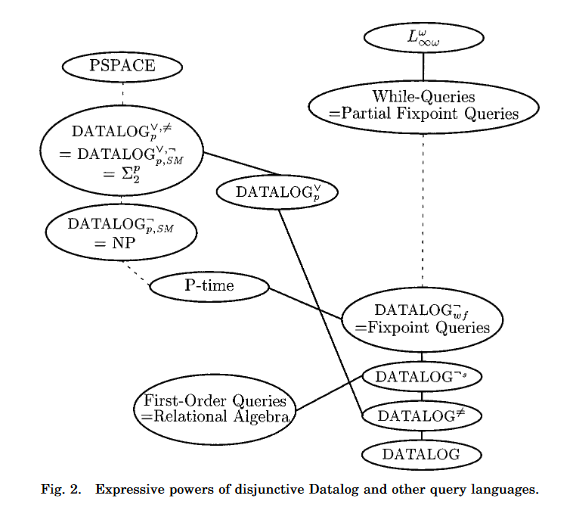
\includegraphics[scale=0.7]{fig/poder-expresivo.png}
\end{figure}

\subsubsection*{Teorema de Ehrenfeucht-Fraisse}
Es una demostración basada en Teoría de Juegos que se usa para determinar si dos estructuras son \textbf{elementalmente equivalentes} (isomorfas). Cuenta con dos jugadores: Spoiler y Duplicator, y dos estructuras (grafos): A y B. Se juega por rondas y en cada una Spoiler elige un nodo de una estructura y en respuesta Duplicator debe elegir uno de la otra. \\
Spoiler busca demostrar que las estructuras son \textbf{distinguibles}, mientras que Duplicator busca lo contrario. Dadas n rondas los grafos son \textbf{indistinguibles} si a partir de los nodos elegidos de cada estructura se tiene un isomorfismo parcial (se mantiene la igualdad y adyacencia). Si para n rondas Duplicator tiene estrategia ganadora decimos que:
\begin{center}
    A $\sim$n B
\end{center}
Ahora, las estrategias se pueden expresar a través de fórmulas de LPO donde la cantidad de rondas se corresponde con la cantidad de cuantificadores. Por ende, si A $\sim$n B luego A y B cumplen las mismas sentencias con n cuantificadores. Generalizado a la LPO:

\textbf{Teorema:} \textit{Una propiedad P no es expresable en la LPO si para todo n natural se pueden hallar dos grafos A y B tales que P sea falsa en A, verdadera en B y A $\sim$n B.}

Hay predicados \quotes{extra-lógicos} en SQL que permiten expandir su poder expresivo: recursión, funciones de agregación y agregamiento, operaciones aritméticas sobre atributos numéricos, store procedures.

\section*{Normalización}
Al diseñar bases de datos la normalización surge como una técnica para tener una \textbf{medida de calidad} sobre sus esquemas (aunque pueda variar según el contexto de uso). Se toma en un nivel conceptual (significado de las relaciones) y uno implementativo (cómo se almacenan físicamente las tuplas). Primordialmente, busca \textbf{preservar la información} y \textbf{minimizar la información almacenada de forma redundante}.

\subsection*{Pautas de diseño}
El proceso de normalización se basa en 4 pautas de diseño que pueden usarse como guía sin necesariamente determinarlo (no siempre son independientes entre sí).
\begin{itemize}
    \item \textbf{Semántica:} Diseñar los esquemas de manera que sea intuitivo entender el significado de sus atributos para evitar confusiones y malos usos. Esto implica no combinar atributos de diversos tipos de entidades y relaciones en la misma relación.
    \item \textbf{Almacenamiento:} Minimizar el espacio ocupado por el diseño evitando anomalías de actualización. Entre ellas tenemos:
    \begin{itemize}
        \item \textbf{Inserción:} La incorporación de una nueva instancia de una entidad está ligada a la existencia de otra o puede producir inconsistencias con datos anteriormente cargados en la relación.
        \item \textbf{Deleción:} El borrado de una instancia produce que se pierda toda la información de otra.
        \item \textbf{Modificación:} Modificar una instancia de una entidad puede volver sus datos inconsistentes con los de las apariciones de una entidad en la relación.
    \end{itemize}
    Al permitir alguna de estas anomalías es preferente que estén debidamente indicadas para su correcta operación. Una razón por la que se suele violar esta pauta es la mejora en el \textbf{rendimiento} subyacente dada por el caso de uso (por la frecuencia de las consultas y actualizaciones puede convenir tener un campo de más pero de rápido acceso).
    \item \textbf{NULL:} Evitar la presencia de valores nulos en las relaciones debido a su variedad de interpretaciones posibles (valor no aplicable, desconocido, concido y ausente). Cuando sean inevitables deben ser la excepción.
    \item \textbf{Tuplas espúreas:} No crear descomposiciones en las que al reconstruir la información usando juntas esta no se corresponda con la original. Esto suele ocurrir cuando en una descomposición no se mantienen las claves de las entidades de la relación. Puede verificarse a través de consultas que usen ambas entidades.
\end{itemize}

\subsection*{Dependencias funcionales (DF)}
Son herramientas formales utilizadas para analizar esquemas que ayuden a detectar algunos de los problemas mencionados. Representadas de la forma $X \rightarrow Y$ donde $X$ e $Y$ son subconjuntos de atributos de la relación, nos dicen que los valores de $Y$ dependen de los de $X$, imponiendo así una \textbf{restricción} sobre las posibles tuplas que se pueden formar. \\
Se especifican según la semántica de los atributos de la relación. Con ello, una \textbf{instancia legal} es aquella que las respeta (también llamada extensión o estado legal). Nótese que sólo con los datos no es posible determinarlas, aunque nos permiten confirmar su existencia o descartarlas.

\subsection*{Proceso de normalización}
Partiendo de las DFs y las claves de cada relación de una DB, podemos aplicarle una serie de tests para certificar si satisface una \textbf{forma normal}. De no hacerlo, se le puede aplicar un \textbf{proceso de normalización} enfocado en minimizar la redundancia y las anomalías de inserción, deleción y modificación para que en una nueva descomposición la DB pase estos tests. Nótese que las formas normales no garantizan un buen diseño de la DB. \\
Tras efectuar este proceso se buscan:
\begin{itemize}
    \item \textbf{Nonadditive Join (SPI):} Garantía de que no se produzcan tuplas espúreas, es decir, se puede recuperar la información original.
    \item \textbf{Preservación de DF (SPDF):} Cada DF estará representada en algún esquema resultante de la descomposición.
\end{itemize}
Lo primero se busca a cualquier costo, mientras que lo segundo es a veces sacrificado. \\
Una DF $X \rightarrow Y$ es \textbf{completa} si al eliminar un atributo de $X$ la dependencia deja de existir. Es \textbf{parcial} si sigue existiendo. Por otra parte, la \textbf{cobertura minimal} $F_M$ de un conjunto de dependencias $F$ es tal que el lado derecho de cada dependencia tiene un sólo atributo y las dependencias son completas. Para formarla debemos descomponer los atributos a derecha, quitar los redundantes a izquierda y eliminar las DFs redundantes (no es conmutativo el proceso).

\subsubsection*{Formas normales basadas en Clave Primaria}
\begin{itemize}
    \item \textbf{1FN:} No deben haber relaciones dentro de relaciones o como atributos dentro de las tuplas. Esto implica que el dominio de los atributos sólo puede ser de valores atómicos (o sea, no pueden ser \textbf{multivaluados}). Para alcanzar esta forma normal suele tomarse el atributo en una nueva relación que tenga como PK a ambos atributos. \\
    Otras opciones involucran expandir la PK (introduciendo posible redundancia) o dividir el atributo en la cantidad de valores que puede tomar (derivando en posibles valores nulos). A través de la aplicación recursiva de 1FN se pueden sacar las \textbf{relaciones anidadas} de una relación.
    \item \textbf{2FN:} Todos los atributos no primos deben depender completamente de la PK de la relación. Para pasar a 2FN basta con descomponer en subesquemas en los que aparezcan los atributos de la PK de los que dependen como parte de su clave.
    \item \textbf{3FN:} Una DF $X \rightarrow Y$ es transitiva si tenemos un conjunto de atributos no primos $Z$ tal que $X \rightarrow Z$ y $Z \rightarrow Y$. Luego, en esta FN ningún atributo no primo debe depender transitivamente de la PK. Para satisfacerla garantizando SPI e SPDF tomamos la cobertura minimal $F_M$ de la relación, formamos los subesquemas $XA$ de cada DF $X \rightarrow A$, unimos los de igual lado izquierdo, agregamos uno con los atributos de una clave si ninguno de los resultantes contiene alguna y eliminamos los esquemas redundantes.
    \item \textbf{BCFN (Boyce-Codd Normal Form):} Toda dependencia funcional no trivial $X \rightarrow A$ de la relación debe tener a $X$ como SK. Es más restrictiva que 3FN y al pasar a esta pueden perderse DFs ya que su proceso se basa en crear subesquemas reemplazando las DFs que violan esta FN.
\end{itemize}

\subsection*{Inferencia}
Una DF es \textbf{inferida} por un conjunto de DFs si se cumple para toda instancia legal de la relación que cumpla con este cojunto. Con esto, la \textbf{clausura} $F^+$ de un conjunto de DFs $F$ son todas las dependencias funcionales que pueden ser inferidas a partir de este. A partir de esta podemos hallar una CK $X$ si $X \rightarrow A$ pertenece y para ningún subconjunto $Y$ de $X$, $Y \rightarrow A$ peretenece ($X$ entonces determina funcionalmente a todos los atributos de la relación).
Podemos calcular $F^+$ aplicando las \textbf{reglas de inferencia} (o \quotes{axiomas de Armstrong}):
\begin{itemize}
    \item \textbf{RI1 (regla reflexiva):} Si $X$ contiene a $Y$ entonces $X \rightarrow Y$.
    \item \textbf{RI2 (regla de incremento):} $X \rightarrow Y$ implica $XZ \rightarrow YZ$.
    \item \textbf{RI3 (regla transitiva):} $X \rightarrow Y$ e $Y \rightarrow Z$ implican $X \rightarrow Z$.
\end{itemize}
Estas crean una clausura \textbf{fiable} (toda DF implicada a partir de $F$ es inferida) y \textbf{completa} ($F^+$ es determinada completamente a partir de $F$ aplicando estos axiomas). Entre sus corolarios tenemos:
\begin{itemize}
    \item \textbf{RI4 (regla de descomposición o proyección):} $X \rightarrow YZ$ implica $X \rightarrow Y$.
    \item \textbf{RI5 (regla de unión o aditiva):} $X \rightarrow Y$ e $X \rightarrow Z$ implican $X \rightarrow YZ$.
    \item \textbf{RI6 (regla pseudotransitiva):} $X \rightarrow Y$ e $WY \rightarrow Z$ implican $WX \rightarrow Z$.
\end{itemize}
\section*{Transacciones}
Son conjuntos de instrucciones que al ejecutarse forman una \textbf{unidad lógica de procesamiento}. Pueden tener uno o más accesos a la DB a través de diversas operaciones: inserción, eliminación, modificación, etc. \\
Las transacciones pueden ser \textbf{read-write} ó \textbf{read-only} según si actualizan o no los ítems de la DB. Los ítems leidos conforman su \textbf{read-set} y los actualizados su \textbf{write-set}. El tamaño de cada uno viene dado por su \textbf{granularidad} (registro, bloque de disco, valor) y esta determina su identificador (número, dirección física). \\
Entre sus operaciones tenemos:
\begin{itemize}
    \item \textbf{read\_item(X):} Se toma la dirección del bloque de disco del ítem X, se copia su contenido al buffer de memoria principal (de no haberlo hecho) y finalmente se copia el ítem X del buffer a la variable X del programa.
    \item \textbf{write\_item(X):} Similar al anterior con la diferencia de que se copia el contenido de la variable X del programa al ítem X del buffer y este es luego almacenado en memoria, según la \textbf{política} de copia de datos a disco (depende de la caché, SO y recovery manager).
\end{itemize}

\subsection*{Propiedades ACID}
En los sistemas de control de concurrencia y recovery procuramos que se cumplan una serie de propiedades:
\begin{itemize}
    \item \textbf{Atomicity:} Las transacciones son unidades atómicas, por lo que se ejecutan en su completitud o no se ejecutan. Depende del subsistema de recovery del DBMS.
    \item \textbf{Consistency preservation:} La transacción al ejecutarse lleva la DB de un estado consistente a otro. Depende de que los programadores cumplan con las restricciones de integridad impuestas, ya que la DB no tiene manera de verificarlo automáticamente.
    \item \textbf{Isolation:} La ejecución de una transacción no debe interferir con la de otra, es decir, debe simular ser aislada incluso al ejecutarse a la vez. Depende del subsistema de control de concurrencia y puede ser de varios \textbf{niveles}: 0 (sin sobreescribir dirty reads), 1 (sin lost updates), 2 (sin lost updates ni dirty reads) o 3 (nivel 2 sin repeatable reads).
    \item \textbf{Durability:} Los cambios aplicados a una DB por una transacción commiteada deben perdurar ante fallos. Depende del subsistema de recovery del DBMS.
\end{itemize}

\subsection*{Subsistema de manejo de transacciones}
Este subsistema del DBMS se conforma de los siguientes módulos:
\begin{itemize}
    \item \textbf{Transaction manager (TM):} Encargado de preprocesar y ejecutar las transacciones en coordinación con el resto. Dentro de ellas, las operaciones tienen un orden fijo y pueden terminar en commit o abort.
    \item \textbf{Scheduler (planificador):} Controla el orden de ejecución de las transacciones en base a una serie de reglas definidas según el paradigma.
    \item \textbf{Recovery manager (RM o log manager):} Encargado de asegurar la durabilidad y atomicidad de las transacciones. Realiza las siguientes operaciones:
    \begin{itemize}
        \item \textbf{RM-Read($T_i$,x):} lee x para la transacción $T_i$.
        \item \textbf{RM-Write($T_i$, x, v):} escribe v en x para la transacción $T_i$
        \item \textbf{Commit($T_i$):} Commitea $T_i$ según la política de recovery.
        \item \textbf{Abort($T_i$):} Aborta $T_i$ según la política de recovery.
        \item \textbf{Restart:} Lleva a la base de datos al último estado commiteado según el log y la política de recovery.
    \end{itemize}
    \item \textbf{Buffer manager (BM):}, tiene un protocolo de operaciones que le dan al Recovery Manager soporte para acceder y modificar la Base de Datos, siendo dichas operaciones:
    \begin{itemize}
        \item \textbf{INPUT(X):} Copia el bloque de disco del ítem X a un buffer de memoria.
        \item \textbf{READ(X, t):} Copia el contenido del ítem X del buffer de memoria a la variable temporal t en memoria local.
        \item \textbf{WRITE(X, t):} Copia el valor de la variable local t al ítem X en un buffer de memoria.
        \item \textbf{OUTPUT(X):} Copia el bloque conteniendo al ítem X del buffer de memoria a disco.
        \item \textbf{FLUSH LOG:} Ordena al buffer manager escribir los registros del log a disco.
    \end{itemize}
    \item \textbf{Cache manager (CM):} Encargado de manejar las transferencias entre el disco y el almancenamiento no volatil. Entre sus operaciones tenemos:
    \begin{itemize}
        \item \textbf{Fetch(X):} Toma un slot vacío c de la caché, copia en este el valor del ítem X de disco, inicializa su dirty bit indicando que puede ser modificado con respecto a disco y actualiza el directorio de esta memoria para señalizar que este slot es ahora ocupado por el ítem X.
        \item \textbf{Flush(X):} Escribe el contenido del ítem X de caché a disco. Se puede efectuar automáticamente si al hacer Fetch(Y) no hay espacio para el ítem Y en caché.
        \item Pin y Unpin
    \end{itemize}
    \item \textbf{Data manager (DM):} Es una entidad que engloba al \textbf{Recovery manager}, \textbf{Cache manager}, a la \textbf{Base de Datos} (no al DBMS, sino a la estructura donde están guardados los datos) y la \textbf{Cache} (como estructura, no como manager).
\end{itemize}
\section*{Control de concurrencia}
Los sistemas que implementan transacciones suelen requerir de respuesta rápida y alta disponibilidad por ser multiusuario con usuarios concurrentes. Algunos ejemplos son los sistemas de reserva de vuelos, transferencias bancarias, procesamiento de tarjetas de crédito y manejo de stock (otros ejemplos: sistemas de reserva de aerolíneas, cajeros electrónicos y supermercados). \\
En la \textbf{multiprogramación} dos o más procesos se ejecutan concurrentemente y si no lo hacen de forma paralela su ejecución es \textbf{intercalada} en una CPU. Aquí hay que atender a una serie de posibles problemas (tomamos $T_1$ y $T_2$ transacciones con $T_1 < T_2$):
\begin{itemize}
    \item \textbf{Incorrect Summary Problem:} $T_1$ modifica $X$ y $Y$, restándole $N$ a $X$ y sumándoselo a $Y$. $T_2$ lee $X$ después de su modificación y $Y$ antes de dicha modificación. Si $T_2$ retorna la suma de ambos, va a devolver $N$ menos de lo que debería porque no llego a ver la suma de $Y$, resultando en una sumarización incorrecta.
    \item \textbf{Lost Update Problem:} $T_2$ lee el valor de un ítem $X$ previo a que $T_1$ lo modifique o lo sobrescribe, y $T_2$ sobrescribe dicho valor sin haber visualizado la escritura final de $T_1$, faltando una actualización en $X$.
    \item \textbf{Temporary Update Problem (Dirty Read):} $T_2$ lee el valor de un ítem $X$ de una $T_1$ que no fue aún commiteada. Esto es un problema ya que potencialmente podría ser abortada.
    \item \textbf{(Non/Un)repeatable Read Problem:} $T_2$ lee el mismo ítem $X$ dos veces y entre ambas lecturas es modificado por $T_1$, dando lugar a diferentes valores.
    \item \textbf{Phantom Read Problem:} $T_2$ realiza más de una lectura sobre una tabla y su conjunto de tuplas es modificado por $T_1$ (ya sea por la aparición/desaparición de tuplas, como por la modificación de tuplas). (nótese que la diferencia con \textbf{Unrepeatable Reads} es que no se modifica un valor, sino que aparecen/desaparecen o modifican tuplas en tablas). 
\end{itemize}


\textbf{Lost Update} es resuelto por cualquier nivel de aislamiento. Para que no se produzcan \textbf{dirty reads}, se debe exigir \textbf{``Read Commited''}, para evitar \textbf{Unrepeatable reads} se exige \textbf{``Repeatable Read''}, y finalmente para que no sucedan \textbf{Phantom Reads} se exige \textbf{``Serializable''} como nivel de aislamiento. 

Existe un final evaluado en esta materia donde se pregunta en que nivel se cubre \textbf{Incorrect Summary}. La respuesta no está en las diapositivas pero la respuesta es deducible y es en el nivel de aislamiento \textbf{``Serializable''}, y ello se debe a que uno puede formular un contraejemplo:

El contraejemplo es el siguiente. Sea $T_1$ y $T_2$ dos transacciones, $T_1$ lee 2 variables, llamémoslas $X$ y $Y$. Si $T_2$ modifica ambas variables, pero $T_1$ lee $X$ de una $T_0$ muy anterior commiteada, y posteriormente lee $Y$ de $T_2$ una vez que $T_2$ commitea, entonces claramente no tenemos \textbf{Lost Update} (porque solo una transacción produjo escrituras, y la otra produjo lecturas, además que no hubo sobre escrituras de un mismo dato, sino escrituras en datos distintos), ni tampoco tenemos un \textbf{dirty read} (ambas variables fueron leídas por $T_1$ estando commiteadas), no tenemos \textbf{Unrepeatable reads} (ambas variables fueron leídas de distintas tuplas), pero si tenemos \textbf{Phantom Read} (ya que entre ambas lecturas, el conjunto de tuplas sobre el que se trabajaba fue modificado), por lo que nuestro \textbf{Incorrect Summary} se transformo en un problema de \textbf{Phantom Read}, y por tanto solo podrá ser resuelto por el nivel más alto de aislamiento. 

Nótese que por esto es importante incluir la modificación de tuplas y no solo la aparición o desaparición de tuplas en la definición de \textbf{Phantom Read}, ya que sin incluirla, este caso no estaría cubriendo el \textbf{Incorrect Summary Problem} y por tanto no sería completamente serializable. Por eso decidí tomar la definición de \textbf{Phantom Read} del siguiente Link, que hace mención de la modificación de tuplas a través de Update de \textbf{SQL}. \href{https://docs.microsoft.com/en-us/sql/odbc/reference/develop-app/transaction-isolation-levels?view=sql-server-ver16}{\textbf{\textcolor{cyan}{Niveles de Aislamiento según Microsoft.}}}

\subsection*{Historia}
Una \textbf{historia} (plan) determina la forma en que se ejecuta un conjunto de transacciones restringiendo que las operaciones sigan su orden si pertenecen a la misma transacción. De allí decimos que que dos operaciones entran \textbf{en conflicto} cuando son de transacciones diferentes, operan sobre el mismo ítem y al menos una es una escritura (no pueden ejecutarse en simultáneo). \\
Además, dadas dos transacciones $T_1$ y $T_2$ decimos que \textbf{$T_1$ lee $X$ de $T_2$} si $T_1$ escribe sobre $X$ y $T_2$ es la última transacción no abortada que había escrito sobre $X$.

\subsubsection*{Definiciones}
\begin{itemize}
    \item \textbf{Equivalencia:} Dos historias son \textbf{equivalentes} si se definen en base al mismo conjunto de transacciones y el orden de las operaciones en conflicto de las transacciones no abortadas es el mismo.
    \item \textbf{Seriabilidad (SR):} Una historia es \textbf{seriablizable} si es equivalente a una serial, lo cual permite satisfacer la propiedad de aislamiento. Podemos verificar si lo es a través de la construcción de un \textbf{grafo de precedencia} (SG(H)), donde cada nodo es una transacción y los arcos dirigidos de $T_i$ a $T_j$ se dan si hay operaciones en conflicto entre ellas y $T_i$ sucede antes que $T_j$. Si el grafo es acíclico, la historia es serializable.
    \item \textbf{Recuperabilidad:} Según las restricciones impuestas, tenemos diferentes niveles:
    \begin{itemize}
    \item \textbf{Recuperable (RC):} Se da si para todo $T_i$, $T_j$ tales que $T_i$ lee de $T_j$ y $T_i$ hace commit entonces $c_i > c_j$.
    \item \textbf{Avoids Cascading Aborts (ACA):} Se da si toda transacción lee de aquellas que hayan hecho commit. De esa forma se pueden evitar los dirty reads sin abortar como en RC.
    \item \textbf{Strict (ST):} Toda transacción lee o escribe en un ítem si la que anteriormente lo había escrito terminó (commit o abort).
    \end{itemize}
    En base a ello: Seriales $\subset$ ST $\subset$ ACA $\subset$ RC.    
\end{itemize}

\subsection*{Paradigmas de planificación}
Atendiendo a los problemas anteriormente mencionados de un sistema concurrente, los schedulers pueden optar al recibir una operación por rechazarla, demorarla o procesarla. Aquellos que favorecen su procesamiento se denotan
 \textbf{agresivos} (mayoría), y si no, \textbf{conservadores} (minoría). Cómo actúen depende de cómo traten a los data ítems: si los bloquean para su uso exclusivo siguen un \textbf{paradigma pesisimista}, mientras que si asumen un comportamiento serializable y actúan en caso de no suceder, \textbf{paradigma optimista}.

\subsubsection*{Paradigma pesimista - Locking}
Para saber si un ítem está disponible para ser usado podemos usar el concepto de \textbf{lock}, que se representa como una variable asociada a este. En su versión \textbf{binaria} un ítem puede bloquearse o desbloquearse a través de las operaciones de lock y unlock. Luego, si una transacción desea operar sobre un ítem debe solicitar un lock sobre este y esperar a que se lo otorguen. Esto hace que sólo una transacción pueda operar sobre el ítem a la vez, incluso si las operaciones son lecturas. \\
Para salvar esta limitación se tiene el \textbf{shared lock (ternario)}, que permite que el lock sea \textbf{exclusivo} (write lock) o \textbf{compartido} (read lock), con sus respectivas operaciones. De ahí, si una transacción desea que pase de uno a otro deberá efectuar una operación de \quotes{upgrade}. \\
Luego, una transacción puede leer un ítem $X$ si solicitó un lock sobre este y no lo ha liberado, y ninguna otra tiene un write lock a la vez. Para la escritura se requiere haber solicitado y no liberado un write lock y que ninguna otra tenga un lock sobre $X$ o haya pedido un upgrade.

\subsubsection*{Two Phase Locking (2PL)}
Decimos que una transacción cumple con el mecanismo \textbf{2PL} si toda operación de lock precede a toda operación de unlock (fases de crecimiento y decrecimiento). Si en una historia legal todas sus transacciones lo cumplen podemos demostrar que la historia es \textbf{serializable} (el algoritmo es correcto). \\
Decimos que una transacción es \textbf{2PL Estricta (2PLE)} si es 2PL y no libera ninguno de sus locks de escritura hasta después de hacer commit o abort. Esto garantiza que una historia sea \textbf{ST} pero no libre de deadlocks. Por otra parte, que sea \textbf{2PL Rigurosa (2PLR)} implica que tampoco los de lectura sean liberados antes.

\subsubsection*{Deadlock}
Es la situación en las historias en que en un grupo de transacciones cada una está esperando a que la otra libere un lock y no puede avanzar. Se pueden prevenir o evitar según la estrategia empleada:
\begin{itemize}
    \item Para \textbf{evitarlos} podemos detectar si existe a través de un \textbf{grafo de espera} (Wait For Graph, WFG(H)) donde para cada transacción en un nodo creamos un arco dirigido a otro si debe esperar a que se libere un lock de su transacción. Cuando su último lock de espera se libera, el arco también. \\
    Si el grafo es cíclico hay deadlocks. De ahí se elige a una \textbf{transacción víctima} siguiendo algún criterio (tiempo de ejecución, variables actualizadas o por actualizar, ciclos en los que aparece, etc.) y se la aborta para reiniciarla posteriormente.
    \item La otra opción es \textbf{prevenirlos} implementando \textbf{timestamps (TS)}, que se le asignan a cada transacción según el momento en que comienzan. Esto hace que si una transacción $T_i$ desea solicitar un lock sobre un ítem bloqueado por $T_j$ se tengan dos estrategias:
    \begin{itemize}
        \item \textbf{Wait-Die:} Si TS($T_i$) $<$ TS($T_j$) se pone a $T_i$ en espera y si no se aborta a $T_i$ para reiniciarla más tarde con el mismo TS.
        \item \textbf{Wound-Wait:} Si TS($T_i$) $<$ TS($T_j$) se aborta a $T_j$ y si no se pone a $T_j$ en espera.
    \end{itemize}
    Otras estrategias involucran establecer un \textbf{tiempo de timeout} (su definición no es trivial), \textbf{No Waiting} (NW) o \textbf{Cautious Waiting} (CW). En la última, si $T_i$ solicita el lock de un ítem bloqueado por $T_j$ se tiene que: si $T_j$ no está bloqueada esperando a otra transacción, $T_i$ se bloquea, y si no se aborta.
\end{itemize}

\subsubsection*{Paradigma optimista - Algoritmo por control de timestamp}
En este mecanismo no hay locking sino que el TM le asigna a cada operación un \textbf{timestamp} (TS, el mismo para las de una misma transacción). Luego para dos operaciones en conflicto se decide su orden según este número (se puede tomar del reloj del sistema o un contador). \\
Cada operación se procesa enviándose al data manager (DM) y se verifica con el planificador usando tres datos de cada ítem $X$: su máximo TS de escritura (\textbf{WT(X)}), su máximo TS de lectura (\textbf{RT(X)}) y su bit de commit (\textbf{C(X)}) que indica si la transacción más reciente que lo actualizó ya hizo commit. Con estos, el planificador asume al verificar una operación que el orden de los timestamps es el orden serial y que cada una pudo haber ocurrido si cada transacción se hubiese realizado instantáneamente en su TS. De no darse este comportamiento, la transacción es \textbf{físicamente irrealizable}.

\subsubsection*{Reglas del planificador}
Si la operación recibida es $r_T(X)$ y:
\begin{itemize}
    \item $TS(T) >= WT(X)$: Si C(X) es True se concede la solicitud y se actualiza RT(X) con el máximo entre TS(T) y RT(X). Si es False se demora $T$ hasta que C(X) sea True o $T$ aborte (previniendo \textbf{dirty read}).
    \item $TS(T) < WT(X)$: La transacción es físicamente irrealizable (\textbf{read too late}).
\end{itemize}
Si en cambio recibe $w_T(X)$ y:
\begin{itemize}
    \item $TS(T) >= RT(X)$ y $TS(T) >= WT(X)$: Se escribe el nuevo valor de $X$, se actualiza WT(X) y C(X) $\leftarrow$ False.
    \item $TS(T) >= RT(X)$ y $TS(T) < WT(X)$: Si C(X) es True se aplica la \textbf{Thomas Write Rule} y se ignora la operación de escritura para evitar la sobreescritura. Si es False, se demora $T$ hasta que la transacción anterior termine.
    \item $TS(T) < RT(X)$: La operación es físicamente irrealizable (\textbf{write too late}).
\end{itemize}
Si recibe $C(T)$, para cada ítem $X$ tal que $WT(X) = TS(T)$ se pone C(X) en True y se prosigue con las transacciones atrasadas por este evento. \\
Finalmente, si recibe $Rollback(T)$ (R(T) o A(T)) cada transacción esperando por un ítem $X$ tal que $WT(X) = TS(T)$ se reinicia y verifica nuevamente. \\
Para los casos en que la operación es físicamente irrealizable, se produce un rollback de la transacción con un nuevo TS. Nótese cómo este planificador evita el problema de \textbf{lost update} al abortar la lectura o ignorando la sobreescritura.

\subsubsection*{Paradigma optimista - Control de concurrencia por multiversión}
Este mecanismo se basa en atacar los problemas de \textbf{read too late} del algoritmo anterior al darle a cada transacción la versión vigente de los data items al momento de su inicio. Esto hace que se guarden tantas \textbf{versiones} como la más antigua vigente de las transacciones activas o commiteadas (no abortadas). \\
Para esto, al ocurrir una escritura $w_T(X)$ (legal) se crea una nueva versión de $X$ como $X_t$ con $t = TS(T)$ en la base de datos. En una lectura $r_T(X)$ se busca $X_t$ tal que $t$ sea el máximo TS menor o igual a TS(T). Esto hace que WT(X) se interprete como el máximo $t$ para el que exista $X_t$. Para RT(X) se guarda un valor $tr$ para cada $Xt$ y si $w_{T'}(X)$ es tal que exsite $X_{t,tr}$ tal que $t < TS(T')$ y $tr > TS(T')$ (write too late) entonces se debe hacer rollback de la transacción. Además, se puede borrar $X_t$ si no existe transacción activa $T$ tal que $TS(T) < t$.

\subsubsection*{Comparación entre los paradigmas}
\begin{itemize}
    \item \textbf{Similitudes:} En ambos puede haber \textbf{starvation} de una transacción y se tiene un \textbf{registro global} para manejar el control de concurrencia de las transacciones: en el pesimista son los locks y en el optimista una serie de timestamps de las operaciones con su bit de commit (agrupados en sets en el caso de implementar validación).
    \item \textbf{Diferencias:} El optimista es mejor si la mayoría de las operaciones son de consulta (escritura) o raramente las transacciones decidan leer y actualizar el mismo elemento de la DB. Locking es más efectivo en situaciones de mayor conflicto. Por ende, los sistemas comerciales suelen establecer un \textbf{compromiso} según el tipo de transacción: si es read-only usan las versiones creadas por read-write; si es read-write usan locking creando versiones de los elementos.
\end{itemize}

\section*{Recuperación}
El DBMS debe procurar que, al recibir una transacción todas sus operaciones sean ejecutadas exitosamente, almacenando sus resultados en la DB (commit), o que ninguna operación tenga efecto sobre ella (abort). Si ocurre una \textbf{falla}, en el primer caso el DBMS debe asegurarse que los cambios pasen a disco y en el segundo, que si ya se realizaron operaciones sus cambios se deshagan ya que pudieron haber dejado a la base de datos con valores inconsistentes. \\
Entre las posibles fallas de un sistema tenemos:
\begin{itemize}
    \item \textbf{Fallo de la Computadora (system crash):} Error de HW, SW o red.
    \item \textbf{Falla en la transacción o sistema:} Error en la lógica de la programación (división por cero) o interrupción del usuario.
    \item \textbf{Errores locales o condiciones de excepción detectadas:} Los datos necesarios de la transacción no fueron encontrados.
    \item \textbf{Ejecución del Control de Concurrencia:} Abort por violar la serialización o producir un deadlock. Estas suelen reiniciarse posteriormente.
    \item \textbf{Falla de disco:} Durante una lectura o escritura.
    \item \textbf{Problemas físicos o catástrofes:} Suministro eléctrico, aire acondicionado, incendio, robo, sabotaje, entre otros.
\end{itemize}
De ellas, salvo las dos últimas, el sistema deberá poder mantener la suficiente información para reestablecerse rápidamente en un modo a prueba de fallas. De esto se encarga el \textbf{subsistema de recovery} del DBMS a través de los módulos cache manager (CM), recovery manager (o log manager) y un archivo \textbf{log} en disco.

\subsection*{Log}
Mantiene un \textbf{registro} de todas las operaciones de las transacciones que afectan a la BD de manera de reestablecer el sistema ante fallas. Es incremental y secuencial, se guarda en disco pero no se salva de fallas a disco ni catástrofes, por lo que períodicamente es preferente guardar una \textbf{copia de seguridad} en otro dispositivo. Su presencia hace que para que una transacción se considere \textbf{commiteada} sus cambios debieron haber sido registrados en el log. \\
Entre los registros que se pueden almacenar en el log tenemos:
\begin{itemize}
    \item \textbf{Start record (\texttt{<START $T_i$>}):} El incio de la transacción $T_i$.
    \item \textbf{Commit record (\texttt{<COMMIT $T_i$>}):} El final exitoso de la transacción $T_i$ indicando que sus cambios deben guardarse permanentemente en la DB.
    \item \textbf{Abort record (\texttt{<ABORT $T_i$>})}: El final no exitoso de una transacción $T_i$, indicando que falló y sus cambios deben ser deshechos de la DB.
    \item \textbf{Update record:} La actualización de un ítem $X$ por parte de la transacción $T_i$.
\end{itemize}
Nótese que una transacción se considera \textbf{incompleta} si no contiene un commit record ni abort record, los cuales sólo pueden estar al final de ella. \\
El \textbf{método de logging} determina la información que guardará el update record en el log y cómo operará el RM ante una falla. Entre ellos tenemos undo logging, redo logging y undo/redo logging.

\subsection*{Garbage Collection Rule}

Una entrada $[T_i, x, V]$ puede ser eliminada del log si pasa una de estas condiciones:

\begin{itemize}
        \item $T_i$ Abortó.
        \item $T_i$ Comiteó, $T_j$ es una transacción posterior a $T_i$, $T_j$ comiteó, y $[T_j, x, W]$ aparece en el log. O sea, si otra transacción comiteó después y modificó dicho valor, por lo que $[T_i, x, V]$ no  es \textbf{el último valor comiteado}.
    \end{itemize}

\subsection*{Undo logging}
Se basa en permitir que las \textbf{transacciones incompletas} escriban a disco y deshacer sus cambios si no llegaron a hacer commit antes de la falla. Aquí los update records son de la forma \texttt{<$T_i$, X, v>} indicando que $T_i$ actualizó el valor de $X$ cuya imagen anterior era $v$. Cada update record se baja a disco antes de bajar el nuevo valor de $X$ y el commit record se baja después de todos los cambios de la transacción, indicando que son válidos. \\
Al producirse una falla:
\begin{enumerate}
    \item Se recorre el log desde el final hacia atrás marcando las transacciones según si se encuentra un commit record o abort record.
    \item Por cada update record \texttt{<$T_i$, X, v>} si se encontró un commit o abort record para $T_i$, saltearlo. Si no, asignar $v$ a $X$.
    \item Agregar un abort record al log por cada $T_i$ incompleta y bajarlos a disco.
\end{enumerate}
Este método es conveniente al tener \textbf{pocas transacciones incompletas} ya que deriva en pocos cambios a deshacer. Además, se pueden ir bajando datos a la DB durante la escritura del log para ahorrar tiempo. No obstante, requiere \textbf{leer todo el archivo de log} y que los ítems se bajen a disco justo después de que la transacción termine, aumentando la cantidad de operaciones de entrada y salida.

\subsection*{Redo logging}
Se basa en tomar las \textbf{transacciones completas} cuyos cambios no llegaron a bajarse a disco. Sus update record son de la forma \texttt{<$T_i$, X, v>} donde la transacción $T_i$ actualizó a $X$ con el valor $v$. Estos se bajan a disco antes que el nuevo valor de $X$ pero el commit record también, de manera de asegurar en el log los cambios a escribir en la BD. \\
Al producirse una falla:
\begin{enumerate}
    \item Se recorre el log una primera vez identificando las transacciones completas e incompletas.
    \item En el segundo recorrido de atrás hacia adelante, por cada update record \texttt{<$T_i$, X, v>} si $T_i$ es incompleta no hacer nada; pero si no asignar $v$ a $X$.
    \item Por cada $T_i$ incompleta agregar un abort record al log y bajarlos a disco.
\end{enumerate}
Nótese que puede optarse por borrar los registros de una transacción abortada o commiteada en caso de haber una más reciente que haya actualizado sus ítems. Sin embargo, en la recuperación \textbf{el archivo de log debe leerse dos veces} y como las transacciones suelen ser completas va a haber muchos cambios a rehacer. A su vez, como los cambios no pueden bajarse a la BD hasta luego del commit es necesario mantener los bloques modificados en un \textbf{buffer}.

\subsection*{Undo/Redo logging}
Es una combinación de los anteriores que se basa en atacar tanto \textbf{transacciones incompletas como completas}. Sus update records son de la forma \texttt{<$T_i$, X, $v_0$, $v_1$>} donde $T_i$ actualizó el valor del ítem $X$ de $v_0$ a $v_1$. Cada uno de ellos se baja a disco antes de acutalizar $X$. Luego se baja su commit record. \\
Con ello, si ocurre una falla:
\begin{enumerate}
    \item Se aplica \textbf{UNDO} a las transacciones incompletas en orden inverso (usando $v_0$ para actualizar el valor de X por cada update record).
    \item Se aplica \textbf{REDO} a las transacciones completas en orden (asignado $v_1$ a $X$ por cada update record).
    \item Agregar un abort record a cada transacción incompleta y bajarlos a disco.
\end{enumerate}
Esto hace que el sistema sea más \textbf{flexible} a los escenarios de fallas, pero para ello debe guardar más información y el trabajo de recuperación es mayor.

\subsection*{Checkpoint}
Considerando que regularmente es necesario bajar los datos del log al disco ya que de expandirse lo suficiente se perdería mucho tiempo en la recuperación, podemos implementar un \textbf{sistema de checkpoints}. Se basa en dos técnicas:
\begin{itemize}
    \item Actualizar el log junto con la lista de transacciones commiteadas y abortadas hasta el momento de manera de indicar las modificaciones escritas y deshechas que no deben realizarse.
    \item Escribir las imágenes posteriores a las modificaciones efectuadas por las transacciones commiteadas o las imágenes previas de las abortadas a disco. Esta es opcional.
\end{itemize}
En base a ello, los mecanismos de checkpoint son:
\begin{itemize}
    \item \textbf{Quiescente:} Este deja de aceptar nuevas transacciones mientras espera a que las activas (las empezadas sin registro de commit o abort) terminen. Luego agrega al log el registro \texttt{<CKPT>} y lo baja a disco (no hay transacciones activas). Recién en ese momento puede aceptar nuevas transacciones. En la recuperación sólo aplica el método \textbf{UNDO} desde el final del log hasta el último checkpoint (el primero encontrado).
    \item \textbf{No quiescente:} Este sigue aceptando transacciones pero efectúa un \textbf{flush} cuando todas las activas a su inicio terminan. Para eso usa el registro \texttt{<START CKPT (...)>} para indicar su inicio en el log con sus transacciones activas y \texttt{<END CKPT>} para indicar que terminaron. \\
    Sus etapas y recuperación varían según el método de logging:
    \begin{itemize}
        \item \textbf{UNDO:} Parte de agregar el registro \texttt{<START CKPT (...)>} al log y bajarlo a disco. Seguidamente, se espera a que estas transacciones terminen, sin restringir que empiecen nuevas. Al terminar se agrega el registro \texttt{<END CKPT>}, bajándolo a disco. \\
        En la recuperación se empieza recorriendo desde el final. En caso de encontrar un \texttt{<END CKPT>} se procede hasta hallar un \texttt{<START CKPT ($T_1$, ..., $T_k$)>}. Seguidamente, se continua recorriendo hasta hallar el \texttt{<START $T_i$>} más antiguo entre las $T_i$ del registro. Finalmente se procede con el método normal.
        \item \textbf{REDO:} Parte similar al anterior, agregando el registro \texttt{<START CKPT (...)>} y bajándolo a disco. Ahora, espera a que se bajen a disco los cambios de todas las transacciones ya commiteadas al momento de iniciar el checkpoint. Finalmente, se agrega el registro \texttt{<END CKPT>} al log y se lo baja a disco. \\
        En la recuperación se indentifica al último checkpoint finalizado correctamente (el último con un \texttt{<END CKPT>} posterior). Luego, desde su registro \texttt{<START CKPT (...)>} se aplica \textbf{REDO} a todas las transacciones que iniciaron luego de su inicio o estaban activas en ese momento.
        \item \textbf{UNDO/REDO:} Agrega al log los registros \texttt{<START CKPT (...)>} y \texttt{<END CKPT>} como en el caso \textbf{REDO}. La diferencia recae en que antes de aplicar \textbf{REDO} sobre las completas aplica \textbf{UNDO} desde el final hasta encontrar el \texttt{<START $T_i$>} más antiguo del último \texttt{<START CKPT (...)>} para las incompletas.
    \end{itemize}
\end{itemize}
\section*{Optimización}
Una \textbf{query} (consulta) tiene muchas formas de ser ejecutada para obtener el set deseado. Cada una define un \textbf{plan} (query plan) y para elegir cuál ejecutar el DBMS cuenta con un módulo llamado \textbf{query optimizer}. \\
Ahora, como encontrar el plan óptimo es un \textbf{problema NP-completo}, el módulo debe emplear otras técnicas para hallarlo en un tiempo razonable. Entre ellas tenemos:
\begin{itemize}
    \item \textbf{Uso de heurísticas:} Se aplican transformaciones del álgebra relacional con la propiedad de mantener los resultados obtenidos. Estas suelen mejorar la performance pero no siempre.
    \item \textbf{Estimación de selectividad:} Se hace uso de la información en la base de datos para estimar el grado de selectividad de la consulta (cantidad de tuplas devueltas). Esto permite darnos una idea de su costo.
    \item \textbf{Índices y tipo de archivo:} El plan elegido depende fuertemente de los índices dispuestos en las tablas y cómo se ordenan físicamente los datos en disco.
\end{itemize}
Una vez obtenido el plan, el code generator se encarga de generar su código correspondiente y el runtime database processor de ejecutarlo.

\subsection*{Métricas de relaciones}
Dada una relación $R$ tenemos una serie de parámetros del catálogo que podemos medir y usar para optimizar una consulta:
\begin{itemize}
    \item \textbf{Bloque:} Porción de datos levantada por cada lectura a disco.
    \item \textbf{LB:} Longitud de los bloques.
    \item \textbf{B$_R$:} Cantidad de bloques ocupados por $R$.
    \item \textbf{FB$_R$:} Factor de bloqueo de $R$, es decir, la cantidad de tuplas de $R$ que entran en un bloque.
    \item \textbf{L$_R$:} Longitud de una tupla de $R$.
    \item \textbf{T$_R$}: Cantidad de tuplas de $R$.
    \item \textbf{I$_{R,A}$}: Imagen del atributo $A$ de $R$, es decir, cantidad de valores distintos de la columna $A$ en $R$.
    \item \textbf{X$_I$}: Altura del árbol de búsqueda (B+) con índice $I$.
    \item \textbf{FB$_I$}: Factor de bloqueo de $I$, es decir, cantidad de tuplas del índice $I$ que entran en un bloque.
    \item \textbf{BH$_I$}: Cantidad de bloques que ocupan todas las hojas del índice $I$.
    \item \textbf{MBxB$_I$}: Cantidad máxima de bloques en un bucket del índice hash $I$.
    \item \textbf{CBu$_I$:} Cantidad de buckets del índice hash $I$.
    \item \textbf{B}: Cantidad de bloques que entran en memoria principal.
\end{itemize}

\subsubsection*{Almacenamiento físico}
Las relaciones se almacenan en \textbf{archivos} y cada tupla tiene asociado un identificador llamado \textbf{rid} (register id), que no es un atributo de la relación. Estos archivos pueden ser:
\begin{itemize}
    \item \textbf{Heap files:} Son el tipo de archivo más simple consistente en una \textbf{colección desordenada} de registros agrupados en bloques. Aquí su \textbf{costo} de exploración completa (scan), búsqueda por igualdad ($A = c$) y búsqueda por rango ($c <= A <= d$) es $BR$ (lineal en la cantidad de bloques). Puede tener páginas para datos y otras para el \textbf{mapa de reserva de índices} (IAM, Index Allocation Table) que sirve para saber dónde están guardados los datos en disco.
    \item \textbf{Sorted file:} Estos mantienen sus \textbf{registros ordenados} según el valor de determinados campos. Si bien su \textbf{costo} de exploración completa sigue siendo $BR$, el de búsqueda por igualdad y búsqueda por rango es $log_2(BR) + [T'/FB_R]$, donde $T'$ es la cantidad de tuplas que cumplen con el criterio de búsqueda (y $FB_R$ la cantidad de tuplas por bloque de $R$).
\end{itemize}

\subsection*{Índices}
Son \textbf{diccionarios de claves} (no necesariamente únicas) asociados a la relación. Cada una se corresponde con una o más columnas (atributos) de ella y su valor asociado es el de sus registros (o tupla). Puede ser el registro completo, su rid a una lista con los rid de todos los registros asociados a ella. \\
De estos se tienen tres tipos:
\begin{itemize}
    \item \textbf{Clustered:} Dicta el \textbf{orden físico} de los datos del archivo, que sólo puede tener uno definido. Se almacenan en forma de \textbf{árbol de búsqueda balanceado} de páginas (B+) de hasta 3 niveles donde sus hojas se corresponden a los datos y cada nodo intermedio referencia en sus filas la dirección física y el valor mínimo de la clave de la página (salvo en la primera que guarda \texttt{NULL} para insertar una fila con clave más baja en la tabla de forma óptima).
    \item \textbf{Non-clustered}: No determinan el orden de los datos y se almacenan en una \textbf{estructura por fuera} de ellos. Se parecen a los anteriores en estructura con la salvedad de que en sus hojas almacenan el valor de la clave y un \textbf{rowid}, que según si se combinan con una heap table o clustered index, es su dirección física o la clave de su fila (respectivamente). En los nodos intermedios se guarda la dirección física de la página con el valor mínimo de clave. Puede guardarse el rowid en caso de haber más de un índice definido.
    \item \textbf{Hash estático:} Se define como una \textbf{tabla de hash} con una cantidad estática de buckets. Es muy útil para realizar búsquedas por igualdad ya que su costo es $MBxB_I$ (cantidad máxima de bloques por bucket). No obstante, para el resto de las operaciones requieren de un barrido lineal (file scan).
\end{itemize}
Los índices pueden ser \textbf{densos} o no según si almacenan una entrada por cada registro en la base de datos o sólo algunos. Además son \textbf{primarios} si guardan registros completos de archivos (sólo uno por tabla) o \textbf{secundarios} si sus valores son rids (puede haber más de uno por tabla).

\subsubsection*{Árbol de búsqueda B+}
Es el \textbf{árbol balanceado} en el que se basan los primeros índices. Siempre tienen una página hoja y otra raíz a menos que la tabla entre toda en una sola. Se busca que \textbf{los datos no se solapen} entre páginas y de sobrar lugar se pueden agregar tablas de índices. \\
Cada nodo interno (y la raíz) tiene una cantidad de hijos y claves dada por un parámetro $d$ (entre $d/2$ y $d$). Las hojas tienen información asociada a la clave de los registros del archivo y se pueden recorrer como $listas doblemente enlazadas$. Esto hace que la estructura sea recomendada para acceder a rangos de claves. \\
Si bien para su exploración completa es necesario un \textbf{file scan}, para las búsquedas cada índice tiene cierta optimización:
\begin{itemize}
    \item \textbf{Clustered:} En la \textbf{búsqueda por igualdad} se recorre el árbol en busca de la primera ocurrencia de la clave. Con ella se busca su registro asociado en el archivo y partir de este punto se lo recorre mientras se hallen ocurrencias de la clave. Esto hace que su costo sea $X_I + [T'/FB_R]$. \\
    Para la \textbf{búsqueda por rango} el costo es el mismo ya que se emplea el msimo método para hallar el primer elemento del rango y recorrer el archivo desde ahí.
    \item \textbf{Non-clustered:} La \textbf{búsqueda por igualdad} es similar al caso clustered pero al llegar a las hojas del árbol se las recorre secuencialmente mientras haya ocurrencias de la clave. Luego, por cada una se leen sus registros asociados. Esto lleva su costo a $X_I - 1 + [T'/FB_I] + T'$. \\
    En la \textbf{búsqueda por rango} el costo es el mismo ya que se sigue el mismo procedimiento para hallar el primer elemento del rango y a partir de este todas sus ocurrencias (leyendo sus registros asociados en el archivo).
\end{itemize}

\subsection*{Operadores del plan de ejecución}
Las consultas se procesan por etapas:
\begin{itemize}
    \item \textbf{Parse:} Validación de la sintaxis de la sentencia SQL con su transformación inicial a árbol de ejecución.
    \item \textbf{Bind:} Vínculo entre los objetos y la carga de metadata.
    \item \textbf{Optimize:} Generación del plan de ejecución.
    \item \textbf{Execute:} Ejecución del plan.
\end{itemize}
En un plan de ejecución, cada nodo es un operador que implementa al menos los métodos:
\begin{itemize}
    \item \textbf{Open():} Se inicializa el operador y se configuran las estructuras de datos requeridas.
    \item \textbf{GetRow():} Se toma una fila del operador.
    \item \textbf{Close():} Se finaliza el operador limpiando las estructuras y datos necesarios.
\end{itemize}
En base a ellos, tenemos dos operadores de acceso a datos:
\begin{itemize}
    \item \textbf{scan:} Barre una estructura. Se denota \textbf{file scan} si recorre todas las entradas de un archivo, o \textbf{index scan}, las de un índice.
    \item \textbf{seek:} Recorre una estructura en base a un índice. Tenemos dos casos:
    \begin{itemize}
        \item Un índice de un \textbf{árbol B+} con un predicado como una conjunción de términos con atributos de un prefijo de su clave (su tupla).
        \item Un índice \textbf{hash} con un predicado como una conjunción de términos con todos los atributos del índice.
    \end{itemize}
    En el caso de un índice non-clustered, al pasar de una hoja a otra estructura se efectúa un \textbf{bookmark lookup} (por rid o clave).
\end{itemize}

\subsubsection*{Juntas:}
Tenemos 3 tipos de operadores de juntas entre relaciones:
\begin{itemize}
    \item \textbf{Nested Loops Join:} Son las más básicas de implementar ya que buscan los elementos recorriendo una tabla a partir de la otra. Son \textbf{efectivas} cuando el inner input es más grande que el outer input y el primero está indexado. Según si el índice forma parte del atributo del join se tiene el \textbf{Index Nested Loop Join} (INLJ) o el \textbf{Block Nested Loop Join} (BNLJ). El costo del primero depende del tipo de índice, siendo el segundo de fuerza bruta. Además el predicado puede no ser de igualdad.
    \item \textbf{Merge Join:} Recorre ordenamente las tablas a través de un scan. Su \textbf{costo} se basa en el algoritmo de ordenamiento (de necesitarse a través de un operador) y el merge (lineal en el tamaño de ambas tablas por condición de igualdad).
    \item \textbf{Hash Join:} Se usa para procesar entradas largas, no ordenadas y sin índices eficientes. Su predicado es de \textbf{igualdad}.
\end{itemize}

\subsubsection*{Otros operadores}
\begin{itemize}
    \item \textbf{Filtro:} Se usan para las condiciones impuestas por la cláusula \texttt{HAVING}, las cuales son eficientes para operar sobre la memoria.
    \item \textbf{Agrupamiento (agregación):} Tenemos \textbf{stream} y \textbf{hash}, donde el primero se usa siempre que no se tenga la cláusula \texttt{GROUP BY} y en caso de hacerlo, los datos deben estar ordenados.
    \item \textbf{Compute Scalar:} Realizan operaciones de conversión, cálculo de datos y otras de cómputo matemático.
    \item \textbf{Union:} Permiten agrupar relaciones y se dividen en \textbf{merge}, \textbf{hash} y \textbf{concat}.
\end{itemize}

\subsection*{Optimizaciones y heurísticas}
\begin{itemize}
    \item \textbf{Algebráicas:} Estas buscan mejorar la performance de la consulta más allá de su representación física aprovechando las propiedades algebráicas del AR:
    \begin{itemize}
        \item Cascada de select/project por conjunción.
        \item Conmutatividad de select/select con respecto a project/producto cartesiano (y la junta)/unión e intersección/select y project con respecto al producto cartesiano (y la junta).
        \item Asociatividad del producto cartesiano, junta, unión e intersección.
    \end{itemize}
    \item La \textbf{materialización} es la escritura de un resultado en disco. Por otra parte, el \textbf{pipelining} se da entre dos operaciones $O_1$ y $O_2$ si las tuplas resultantes de la primera pasan a través de un \textbf{stream} en memoria a la segunda. Esto hace que se ahorre el costo de output de $O1$ y de input de $O_2$. No es aplicable a operaciones que necesitan todas las relaciones de antemano, como las juntas.
    \item La \textbf{integridad referencial} permite evitar consultar a una tabla a través de juntas.
    \item Considerar sólo \textbf{árboles sesgados a izquierda} permite limitar los árboles candidatos a analizar.
    \item Al descomponer las \textbf{selecciones conjuntivas} podemos aprovechar los índices de cada relación por separado.
    \item Tomar las selecciones lo más cercano posible a las hojas del árbol reduce la cantidad de datos a materializar al seleccionar prematuramente las tuplas que nos interesan.
    \item Reemplazar \textbf{productos cartesianos} seguidos de selecciones por juntas.
    \item Descomponer las listas de atributos de proyecciones y llevarlas lo más cerca posible de las hojas.
    \item Los \textbf{hints} son instrucciones para el motor de búsqueda para cambiar su operación. Se especifican a través de la cláusula \texttt{OPTION} y sólo cambian su procesamiento, no su semántica (retornar rápidamente una serie de filas, buscar usando un índice en específico, recompilar una consulta, optimizar en base a un parámetro dado o \textit{parameter sniffing}, entre otras).
    \item Para comparar y analizar las implementaciones de una consulta tenemos las \textbf{estadísticas}. Entre sus métricas, muestran la distribución de los datos en un histograma contando límites por paso, rango de valores, cantidad estimada promedio, valores distintivos y cantidad de duplicados promedio.
    \item Para optimizar lecturas se pueden utilizar los atributos buscables a través de índices (\textbf{SARGable}: search-ARGument-table). Estos se aplican sólo cuando los predicados tienen condiciones de inclusión. En los índices compuestos depende del predicado de su primera columna.
    \item La \textbf{cobertura de un índice} permite guardar partes selectivas en base a un criterio dado y con ello retornar la información necesaria o que se pueda llegar a usar en el futuro. También se puede filtrar el indexado para, por ejemplo, tomar todos los valores no nulos y así recorrer la tabla más rápidamente.
\end{itemize}

\section*{Long duration transacions}
Son aquellas transacciones que caen dentro de dos escenarios:
\begin{itemize}
    \item Modifican una \textbf{cantidad muy grande de registros} de la base de datos. Si se ejecutasen como una sola transacción tardarían mucho tiempo en ejecutarse y requerirían almacenar mucha información para hacer rollback.
    \item Deben \textbf{acceder a diferentes bases de datos} para ejecutarse.
\end{itemize}
Para tratarlas definimos una \textbf{saga} como una colección de acciones que juntas conforman a la transacción. Esta consiste además de un \textbf{grafo dirigido} donde cada nodo es una \textbf{acción}, se tienen los nodos terminales Abort y Complete (no salen ejes de ellos), y una marca del nodo inicial. \\
Con esto, cada camino del grafo representa un \textbf{curso de acción} (secuencia de acciones) que puede llevar a $Abort$ ó $Complete$. Cada acción puede verse como una transacción y para cada una se define su \quotes{transacción de compensación} como aquella que al ejecutarse permite revertir la base al estado anterior a ejecutarse su transacción correspondiente (para la acción $A$ se define como $A^{-1}$). \\
Entonces, si al ejecutar un curso se llega a $Abort$ se usan las transacciones de compensación de sus acciones en el orden inverso para deshacer sus cambios de la base de datos. Si en cambio se llega a $Complete$ los cambios se pueden mantener en la base.
\section*{Bases de datos distribuidas (DDB)}
Se definen como colecciones de BDs \textbf{lógicamente relacionadas} y \textbf{distribuidas} a través de una red de computadoras. Son manejadas por un \textbf{DDBMS} que busca hacer transparente la distribución al usuario y que sus nodos cumplan con una serie de características. \\
Dada una consulta su estrategia de ejecución depende del \textbf{tipo y la topología de la interconexión} entre los nodos de la red (LAN, WAN, conexión directa, conectividad). También depende de la \textbf{forma} en que esté distribuida la información (dada una junta debemos atender a la cantidad de datos que deben ser transeridos).



\subsection*{Fragmentación}
Los \textbf{fragmentos} son las partes resultantes de dividir la DB en unidades lógicas. La fragmentación puede ser:
\begin{itemize}
    \item \textbf{Horizontal (sharding):} Subdivisión en \textbf{subconjuntos de tuplas} de la relación original. Es análoga al operador \texttt{SELECT} y de comprender a todas las tuplas se denomina \textbf{completa} (puede ser disjunta). Su reconstrucción viene dada por \texttt{UNION}. Aumenta el performance de las escrituras y lecturas distribuyendo la carga en distintos nodos, pero reduce el performance de operaciones analíticas al requerir \texttt{UNIONS} cuando se quiere todos los datos de la tabla (ver \hyperlink{olap}{OLAP} y \hyperlink{oltp}{OLTP}).
    \item \textbf{Vertical:} Subdivisión en subrelaciones dadas por un \textbf{subconjunto de columnas} de la original. Es análoga al \textbf{proyector} y si cada atributo está en al menos una proyección y todas comparten sólo la PK se denomina \textbf{completa}. La reconstrucción viene dada por \texttt{OUTER JOIN}. Aumenta el performance de las lecturas y escrituras ya que distribuye la carga en distintos nodos cuando se trata de accesos a pocas columnas, pero a costa que las operaciones que requieran el uso de todas las columnas se vean ralentizadas por la necesidad de realizar \texttt{JOINS}.
    \item \textbf{Mixta:} Combinación de las dos anteriores que puede reconstruir la relación con las operaciones en el orden apropiado.
\end{itemize}
Un \textbf{esquema de fragmentación} de una DB es un conjunto de fragmentos que incluye a todos sus atributos y tuplas, y permite reconstruirla con la secuencia de operaciones apropiada. Por otra parte, un \textbf{esquema de asignación} describe la ubiación de los fragmentos en los nodos de la DDB y de estar uno en más de un lugar se denomina \textbf{replicado}.

\subsection*{Replicación}
Las \textbf{replicas} son copias de los datos que permiten aumentar su disponibilidad y confiabilidad. Según su nivel, la replicación es:
\begin{itemize}
    \item \textbf{Total:} Todos los nodos tienen copias de la DB. \\
    \textbf{Ventajas:} El sistema puede continuar operando si al menos uno está disponible y mejora el rendimiento de lecturas. \\
    \textbf{Desventajas:} El rendimiento de escrituras empeora y las técnicas de control de concurrencia y recuperación son más costosas.
    \item \textbf{Nula:} Caso adverso al anterior en que ningún elemento está replicado. \\
    \textbf{Ventajas:} Las escrituras son menos costosas y no requieren de tanto control de concurrencia ni recuperación. \\
    \textbf{Desventajas:} Tiene múltiples puntos de falla y cuello de botella para lecturas.
    \item \textbf{Parcial:} Algunos elementos se replican y otros no, distribuyéndose a sitios particulares. Esta depende de las metas de disponibilidad, performance y el tipo de transacciones de cada sitio del sistema. La descripción de la replicación viene dada por el esquema de replicación.
\end{itemize}

\subsection*{Transparencia}
Se basa en \textbf{ocultar los detalles} de implementación a los usuarios finales. Si es \textbf{total}, la visión del usuario es la de una DB centralizada donde se centra en la \textbf{independencia} entre datos lógicos y físicos (con el compromiso del sobrecosto de proveerla). Más específicamente, podemos ver distintos \textbf{Tipos de Transparencia} para las DBs distribuidas:
\begin{itemize}
    \item \textbf{Organización de los datos:} Cómo están distribuidos los datos a través de la red. Se divide en transparencia de \textbf{ubicación} (ejecutar una tarea independientemente de dónde estén los datos) y de \textbf{nombres} (tras asociar un nombre a un objeto no hacen falta datos adicionales para ubicarlo).
    \item \textbf{Fragmentación:} El usuario \textbf{se libera de conocer detalles sobre la fragmentación} de los datos. Esa transparencia puede ser para la fragmentación \textbf{horizontal}, \textbf{vertical}, o \textbf{ambas}.
    \item \textbf{Replicación:} El usuario \textbf{se libera de conocer detalles sobre la replicación} de los datos, \textbf{de su ubicación} y la razón por la que fueron replicados, sin embargo \textbf{puede} llegar a \textbf{ser configurable}.
    \item \textbf{Otras Transparencias:} Como de \textbf{Diseño o Ejecución}, que \textbf{lo liberan al usuario de entender donde o cómo se procesan las queries}, y como esta diseñada la misma en y entre los nodos.
\end{itemize}

La \textbf{transparencia}  tiene la ventaja de proveer una visión de la Base de Datos como si fuera \textbf{centralizada}. Pero tiene el problema de no permitir reflejar características deseables del \textbf{DDBMS}.
Por tanto la transparencia \textbf{debe poder ser configurable}, o \textbf{debe haber un compromiso entre la facilidad de uso} y \textbf{el sobrecosto de proveer transparencia}.

\subsection*{Características esperables}
\begin{itemize}
    \item \textbf{Disponibilidad y confiabilidad:} Se refieren a la \textbf{probabilidad} de que un sistema se encuentre continuamente disponible u operando en un determinado intervalo de tiempo (respectivamente, aunque los términos se usen de forma indistinta). Ante las fallas del sistema, un sistema \textbf{confiable} puede:
    \begin{itemize}
        \item \textbf{Enfatizar su tolerancia a las fallas}, reconociendo que pueden ocurrir y diseñar mecanismos que las detecten y las remuevan antes de que ocurran.
        \item \textbf{Asegurar la ausencia de fallas} en el sistema final mediante procesos de desarrollo que incluyen control de calidad y testing.
    \end{itemize}
    En el caso de los DDBMSs, estos deben \textbf{tolerar fallos de sus componentes subyacentes} sin alterar los pedidos de sus usuarios ni la consistencia de la base. El RM se encarga de tratar fallas en las transacciones, hardware y comunicaciones en las redes.
    \item \textbf{Escalabilidad y tolerancia a la partición:} La primera se refiere a la medida en que un sistema puede \textbf{expandirse} mientras continúe operando ininterrumpidamente. Puede ser \textbf{horizontal} (cantidad de nodos del sistema distribuido) o \textbf{vertical} (capacidad de un nodo individual). \\
    La segunda implica que el sistema pueda seguir operando aún cuando la red se particione.
    \item \textbf{Autonomía:} La medida en que los nodos individuales de una DDB puedan operar \textbf{independientemente}. Se busca que tenga alto grado y hay de varios tipos:
    \begin{itemize}
        \item \textbf{Diseño:} Independencia del uso del modelo de datos/técnicas de gestión de transacciones entre los nodos.
        \item \textbf{Comunicación:} Medida en la que los nodos deciden compartir o no información con otros.
        \item \textbf{Ejecución:} Acciones \quotes{a gusto} del usuario.
    \end{itemize}
\end{itemize}

\subsubsection*{Teorema CAP}
Publicado en 1998 y presentrado por Eric Brewen en el año 2000, establece que cualquier sistema que comparta datos a través de la red puede cumplir con a lo sumo dos de las siguientes propiedades:
\begin{itemize}
    \item \textbf{Consistency:} Toda lectura devuelve la escritura más reciente del ítem.
    \item \textbf{Availability:} Todo pedido recibe una respuesta, pero sin el anterior ítem, no se garantiza que esta respuesta sea la de la última escritura. Pero sí garantiza que no es errónea o un código de error.
    \item \textbf{Partition tolerance:} El sistema sigue funcionando a pesar de la perdida de una cantidad arbitraria de paquetes (mensajes) o nodos en la red (incluso aunque los pierda todos). La idea es que si decide seguir con la operación, puede perder consistencia por no disponer de la información que el nodo caído o incomunicable dispone, o puede arriesgar disponibilidad si decide cancelar la operación o retrasarla (porque puede terminar retrasándola infinitamente).
\end{itemize}
Según Brewen, el objetivo del teorema debe enfocarse en encontrar el balance entre consistencia y disponbilidad mientras se encuentre la forma de manejar las particiones de la red, considerando cómo recuperarse ante eventuales fallas. Para lo segundo, el sistema debe detectar la partición, entrar en modo \quotes{particionado} y luego recuperar el modo anterior.

\subsubsection*{Propiedades BASE}
Son las propiedades que cumplen las DBs NoSQL (de las cuales muchas incorporan funcionalidades de DDBs) y son mucho más laxas, o débiles, que las propiedades \textbf{ACID} (las cuáles también son deseables en una DDB). Estas son:
\begin{itemize}
    \item \textbf{Basic Availability:} El sistema debe garantizar disponibilidad en términos del teorema \textbf{CAP} incluso cuando ocurren fallas (si se produce una falla, en el peor de los casos la Base de Datos se reserva la posibilidad de particionarse). No obstante, esta disponibilidad no garantiza consistencia, las lecturas puede no leer la última escritura, y la escritura puede no persistir si se encuentran conflictos no reconciliables. Esto puede lograrlo a través de una base de datos \textbf{altamente distribuida}, en donde no se guarde una sola copia con tolerancia a fallas sino múltiples réplicas en discos. De esa forma, una falla que inhabilita el acceso a un grupo de datos no necesariamente lo hace a toda la DB. 
    \item \textbf{Soft-state:} El estado de la DB puede cambiar a lo largo del tiempo incluso sin intervención externa. Esto significa que en un momento dado no necesariamente habrá una única \quotes{versión} de cada dato y la \textbf{consistencia} debe ser manejada por los desarrolladores, no el DBMS.
    \item \textbf{Eventual consistency:} El sistema garantiza que posterior a la ejecución de escrituras, el sistema converge después de un tiempo no determinado, a un estado donde cualquier lectura de ese ítem de datos siempre retorne el mismo valor, recalcando de vuelta, que los conflictos de concurrencia quedan en manos de los desarrolladores y no del DBMS.
\end{itemize}


\subsubsection*{Ventajas de las DDBs}
\begin{itemize}
    \item Permiten mejorar sencilla y flexiblemente el desarrollo de aplicaciones, debido a la transparencia de control y distribución de los datos.
    \item Aumentan la disponibilidad al aislar sus fallas a su sitio de origen.
    \item Mejoran la performance al fragmentar y replicar los datos, dando nuevas oportunidades de conseguir escalabilidad horizontal (distribuyendo la carga entre nodos) y mantener cerca los datos necesitados (en nodos geográficamente cercanos a dónde se realice la consulta).
\end{itemize}

\subsection*{Control de concurrencia (CC) en DDBs}
Este subsistema se encarga de \textbf{mantener la consistencia} entre las copias de un data ítem en la DB (mientras intenta mantener el resto de las propiedades de las bases centralizadas). Para ello se puede usar la técnica de \textbf{locking} en donde para cada ítem se designa una copia como \textbf{distinguida} y los pedidos de lock y unlock son enviados a ella. \\
Según su ubicación, se tienen diferentes variantes:
\begin{itemize}
    \item \textbf{Sitio primario:} Un  único sitio es \textbf{distinguido} y encargado de procesar las transacciones. Si le otorga el lock a un nodo, puede acceder a cualquier copia de dicho valor. El DDBMS debe asegurarse que al modificar un valor, este se refleje en todas las copias  de dicho valor. \\
    \textbf{Ventajas:} Es una extensión del esquema centralizado y si las transacciones cumplen con el enfoque 2PC la seriabilidad está garantizada. \\
    \textbf{Desventajas:} Hay cuello de botella en el único sitio así como un único punto de falla que puede paralizar al sistema.
    \item \textbf{Sitio primario + backup:} Similar al anterior pero con un \textbf{sitio adicional de backup} para reemplazar al primario en caso de fallar. \\
    \textbf{Ventajas:} Simplifica el proceso de recovery del sitio primario. \\
    \textbf{Desventajas:} La performance de locking disminuye y persiste el problema del cuello de botella.
    \item \textbf{Copia primaria:} Permite que los sitios que almacenan las copias \textbf{sean encargados de procesar las Transacciones y locks}, en vez de tener un Sitio Primario que se encargue de todo. Entre los que tienen la copia de un data item, \textbf{uno} es seleccionado como \textbf{distinguido}, y se encarga de los locks \textbf{de dicho data item}. \\
    \textbf{Ventajas:} Ataca el problema del cuello de botella y el único punto de falla del sitio primario. De combinarse con backups, se puede mejorar su disponibilidad y confiabilidad (aunque con cierto costo adicional). Además, la caída de un nodo solo afecta a las transacciones que pidieron locks en data items de dicho nodo.\\
    \textbf{Desventajas:} La complejidad del control de concurrencia es muchísimo mayor al no parecerse a sus contrapartes centralizadas, y el uso de la red para algoritmos de votación y decisión va a ser mayor que en casos de Sitio Primario.
\end{itemize}

\subsubsection*{Elección de nuevo coordinador}
Al suceder una \textbf{falla}, en los casos sin backup las transacciones que acceden a los datos del sitio afectado deben ser abortadas y reiniciadas, mientras que de haber backup estas son suspendidas hasta ser designados estos sitios como primarios. Si ambos fallan puede iniciarse un \textbf{proceso de elección} de un nuevo coordinador desde un sitio Y:
\begin{enumerate}
    \item El coordinador se considera \textbf{fallido} si el sitio $Y$ intenta reiteradamente comunicarse con él y no lo logra.
    \item Luego, este sitio envía a todos los nodos activos que será el nuevo coordinador.
    \item De recibir la mayoría de los votos positivos, se lo declara como tal. Esto resuelve los casos en que más de un sitio desea ser coordinador a la vez.
\end{enumerate}

\subsubsection*{Votación}
Alternativamente a la copia distinguida, se puede hacer un \textbf{pedido de lock(X)} a todos los sitios con el ítem $X$. De allí, cada copia puede aceptarlo o rechazarlo. Si recibe la mayoría de aprobaciones en un cierto período de tiempo, les avisa a todas las copias que tomó el ítem. Si no, cancela el pedido y les informa de la cancelación. \\
\textbf{Ventajas:} Es un método de CC \textbf{realmente distribuido} por compartir la decisión entre sus nodos.
\textbf{Desventajas:} Genera mucho tráfico de mensajes y de caerse nodos durante la votación el algoritmo puede acomplejizarse.

\subsubsection*{Catálogo}
Es una DB que contiene la \textbf{metadata} del DBMS, además de lo que ya vimos (meta data sobre las tablas, usuarios, vistas, y todo objeto de la Base de Datos), pero en el caso particular del DDBMS, también tiene la información de la \textbf{fragmentación, asignación de fragmentos y replicación de los datos}. Su administración debe tener autonomía de sitio, vistas y distribución y replicación de los datos. Su \textbf{esquema} puede ser:
\begin{itemize}
    \item \textbf{Centralizado:} Se almacena por completo en un sitio. \\
    \textbf{Ventajas:} Su implementación es sencilla. \\
    \textbf{Desventajas:}
    \begin{itemize}
        \item Tiene poca confiabilidad, disponbilidad y autonomía.
        \item Centraliza la distribución de la carga de procesamiento.
        \item Los locks pueden producir un cuello de botella en caso de haber muchas escrituras.
    \end{itemize}
    \item \textbf{Totalmente replicado:} Cada sitio tiene una copia completa del catálogo. \\
    \textbf{Ventajas:} Puede responder a las consultas localmente. \\
    \textbf{Desventajas:} Las actualizaciones deben ser transmitidas a todos los sitios, por lo que se requiere de un esquema centralizado 2PC para mantener la consistencia y las aplicaciones de muchas escrituras, incrementando así el tráfico de la red.
    \item \textbf{Parcialmente replicado:} Cada sitio tiene la información completa del catálogo de los datos almacenados localmente en el sitio. Además pueden almacenar en caché copias de entradas de otros sitios (no necesariamente actualizadas). Luego, el sistema debe registrar para cada entrada del catálogo los sitios en que se creó el objeto y en donde están sus copias para propagar los cambios de ellas al original.
\end{itemize}

\subsection*{Recuperación en DDBs}
Este subsistema debe atender a dos principales problemas:
\begin{itemize}
    \item \textbf{Fallos en sitios y comunicaciones:} A partir de un sitio $X$ es difícil determinar si un sitio $Y$ se encuentra \textbf{caido} sin intercambiar una gran cantidad de mensajes. En efecto, la falta de respuesta de $Y$ podría deberse además a una falla en la comunicación que hace que no haya recibido el mensaje o no haya podido enviarlo.
    \item \textbf{Commit distribuido:} Cuando una transacción actualiza un valor en varios sitios, no puede commitearlo hasta asegurarse que sus efectos no se perderán en ninguno de ellos (log). Para asegurar la correctitud frente a este problema se suele usar el \textbf{protocolo 2PC}.
\end{itemize}

\subsubsection*{Gestión de transacciones distribuidas}
En las DDBs tenemos varios \textbf{módulos} encargados de garantizar las propiedades \textbf{ACID}: gestor global de transacciones, local de transacciones, de CC y de recovery. El primero actúa en el sitio de origen de la transacción y le pasa la operación al de CC. Este se encarga de manejar los locks y hasta adquirirlo bloquea a la transacción. Tras obtenerlo, el runtime processor ejecuta la operación y luego libera el lock y le avisa al gestor de transacciones del resultado.

\subsubsection*{Protocolo 2PC:}
En este actúan los gestores de recovery (global y local con su información correspondiente) y el TM del nodo coordinador de la operación a realizar. Se divide en dos fases:
\begin{itemize}
    \item \textbf{Primera fase:} El coordinador le \textbf{avisa a todos} los nodos que estén listos para realizar el commit (o abort) y espera recibir la mayoría de aprobaciones para pasar a la siguiente fase (dentro de un tiempo de timeout). Si no lo hace, aborta la operación.
    \item \textbf{Segunda fase:} El coordinador les dice a todos los nodos que va a \textbf{ejecutarse el commit (o abort)} y espera su respuesta positiva dentro de un tiempo de timeout (si no cancela la operación). Sin embargo, si el \textbf{coordinador falla} tras solicitar el lock, el resto de los nodos pueden quedarse permanentemente bloqueados.
\end{itemize}
La respuesta a esto es el \textbf{protocolo 3PC} en el que se agrega una \textbf{fase intermedia} de reconocimiento con tiempo de timeout que causa abort entre la primera y la segunda, y commit entre la segunda y la tercera para estos sitios y evita que se bloqueen.

\subsection*{Gestión de consultas distribuidas}
El procesamiento de las consultas se divide en etapas:
\begin{enumerate}
    \item \textbf{Mapeo:} Se pasa la consulta SQL a AR basándose en el esquema conceptual global y se normaliza y reestructura de manera similar al caso centralizado.
    \item \textbf{Localización:} Se mapea la consulta resultante a múltiples fragmentos individuales en base a la información de distribución y replicación de datos.
    \item \textbf{Optimización de la consulta global:} Se selecciona una estrategia de una lista de candidatas cercanas a la óptima en base a algún criterio: tiempo, costo total, comunicación, entre otros.
    \item \textbf{Optimización de la consulta local:} Se ejecuta en todos los nodos de la DDB con técnicas de optimización centralizadas.
\end{enumerate}

\subsubsection*{Semijoin}
En la tercera etapa, un gran costo a considerar es el de la cantidad de datos a transferir. Una manera de mitigarlo es intentar reducir la cantidad de tuplas de una relación antes de la transferencia. Así, el semijoin consiste en \textbf{enviar sólo las columnas de la junta}, realizarla y de su resultado retornarla junto con los atributos necesarios para completar la consulta. \\
\textbf{Ventaja:} Si sólo una pequeña parte de la relación participa en la junta se puede minimizar la transferencia de datos. \\
\textbf{Desventaja:} Es una heurística y puede fallar.

\subsection*{Tipos de DDBs}
Los sistemas de DDBs pueden diferir según el grado de:
\begin{itemize}
    \item \textbf{Homogeneidad:} Si todos los servidores y usuarios hacen uso del mismo software. Aquí la \textbf{heterogeneidad} puede surgir por diferencias en:
    \begin{itemize}
        \item \textbf{Modelo de datos:} Pueden diferir en su modelo relacional, objetos o archivos (por ejemplo, la misma información puede ser tratada como un atributo o una relación). Sobre esto es necesario un mecanismo inteligente de procesamiento de consultas que relacione la información basándose en metadata.
        \item \textbf{Restricciones:} Varían de sistema a sistema y deben ser tratadas por el esquema global.
        \item \textbf{Lenguaje de consultas:} Dentro del mismo modelo de datos puede tener diferentes versiones.
    \end{itemize}
    También puede haber \textbf{heterogeneidad semántica} si hay diferencias en el significado, interpretación y uso de los datos, gracias a la autonomía de diseño. Se puede tratar con \textbf{software variado} que administre las consultas y transacciones desde la aplicación global a cada DB y visceversa: middleware, application servers, enterprise resourse planning, modelos y herramientas para la \textbf{integración e intercambio de datos} y \textbf{acceso/consulta a datos basado en ontologías}.
    \item \textbf{Autonomía local:} Cuánto depende cada sitio del resto para funcionar como un DBMS por separado. Tenemos de varios tipos:
    \begin{itemize}
        \item \textbf{Comunicación:} Capacidad de decidir cuándo comunicarse con el resto.
        \item \textbf{Ejecución:} Capacidad de un componente de la DB de ejecutar operaciones sin interferir con las del resto y decidir su orden.
        \item \textbf{Asociación:} Capacidad de decidir si compartir y cuánto su funcionalidad y recursos.
    \end{itemize}
\end{itemize}
De aquí se derivan \textbf{FDBS} y \textbf{p2pDBS}, en los que cada servidor es independiente y autónomo con usuarios locales propios, transacciones locales y un DBA (alto grado de autonomía). En el primero hay cierto \textbf{esquema global de la federación} de bases de datos, mientras que en el segundo cada nodo se construye \textbf{a medida que se lo necesita}. Como sus nodos son heterogéneos, es necesario un \textbf{lenguaje canónico} para traducir las consultas.

\subsubsection*{Arquitecturas paralelas y distribuidas}
Dentro de las arquitecturas de \textbf{sistemas multiprocesador} tenemos las de:
\begin{itemize}
    \item \textbf{Memoria compartida:} Múltiples procesadores que comparten memoria primaria y tienen almacenamiento secundario (disco).
    \item \textbf{Disco compartido:} Múltiples procesadores que comparten almacenamiento secundario pero comparten su memoria primaria.
    \item \textbf{Shared-nothing:} Cada procesador tiene su propia memoria y disco. Se comunican a través de redes de alta velocidad. Se busca cierta simetría y homogeneidad entre los nodos.
\end{itemize}
De estas se derivan tipos particulares de arquitecturas:
\begin{itemize}
    \item \textbf{Parallel DBMS (PDBMS):} Son un caso particular de las distribuidas usadas en la industria donde los nodos se encuentran \textbf{físicamente cerca} y se conectan entre sí a través de una \textbf{red local} de alta velocidad. Esto hace que su costo de comunicación sea bajo y puedan implementarse con los 3 tipos mencionados de arquitectura multiprocesador. Su principal diferencia con las distribuidas reside en su \textbf{modo de operación}.
    \item \textbf{Distribuidas puras:} Cada nodo está en un \textbf{sitio diferente} y se comunican a través de una \textbf{red} con un costo no despreciable. Se basan en la arquitectura \textbf{shared-nothing} y tienen un esquema conceptual global y uno interno a cada nodo que junto con el catálogo permiten imponer restricciones y optimizar las consultas locales y globales.
    \item \textbf{3-Tier:} Se desarrollan en el contexto de arquitecturas cliente-servidor y se separan en 3 capas:
    \begin{itemize}
        \item \textbf{Presentation:} La interfaz que interactúa con el usuario.
        \item \textbf{Application:} La encargada de manejar la lógica de negocios de la aplicación.
        \item \textbf{Database Server:} La encargada de manejar, procesar y retornar los pedidos de consulta y actualizaciones de la capa de aplicación.
    \end{itemize}
    Aún así, las funcionalidades DDBMS puede dividirse de diferentes maneras. Más en detalle, la capa de aplicación debe primordialmente encargarse de:
    \begin{itemize}
        \item Generar un \textbf{plan de ejecución distribuido} para las consultas y transacciones y supervisar su ejecución.
        \item Asegurar la \textbf{consistencia} entre réplicas con técnicas de control de concurrencia distribuida.
        \item Asegurar la \textbf{atomicidad} de las transacciones globales, ejecutando un recovery global en caso de producirse una falla.
    \end{itemize}
    Esta capa no siempre puede operar con transparencia de distribución, es decir, sin especificar los sitios en que residen los datos de las consultas o transacciones.
\end{itemize}

\begin{figure}[H]
    \centering
    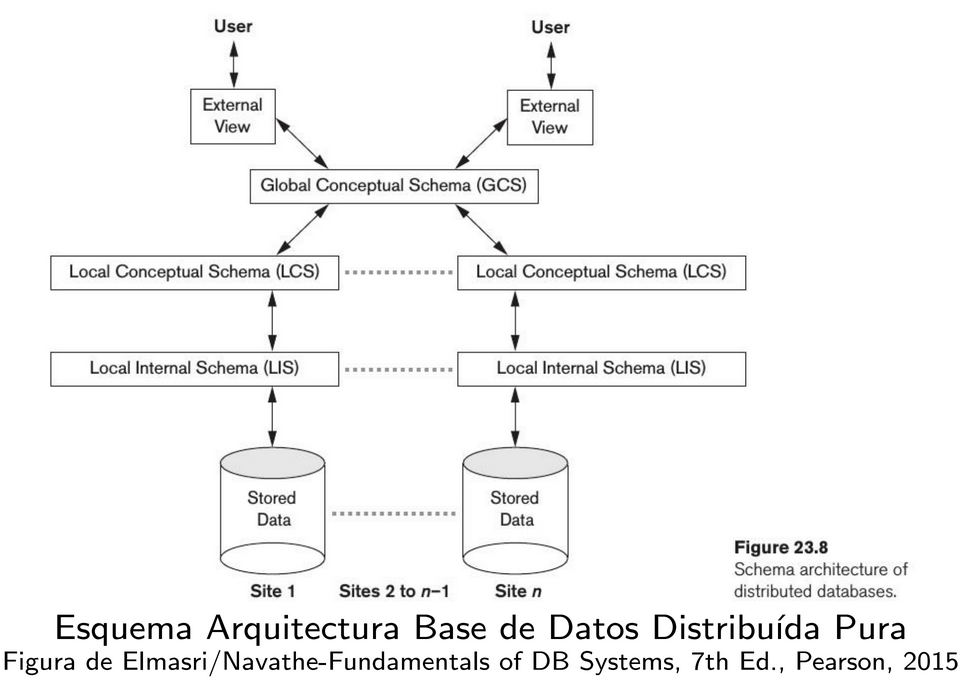
\includegraphics[scale=0.45]{fig/arquitectura-distribuida-pura.png}
    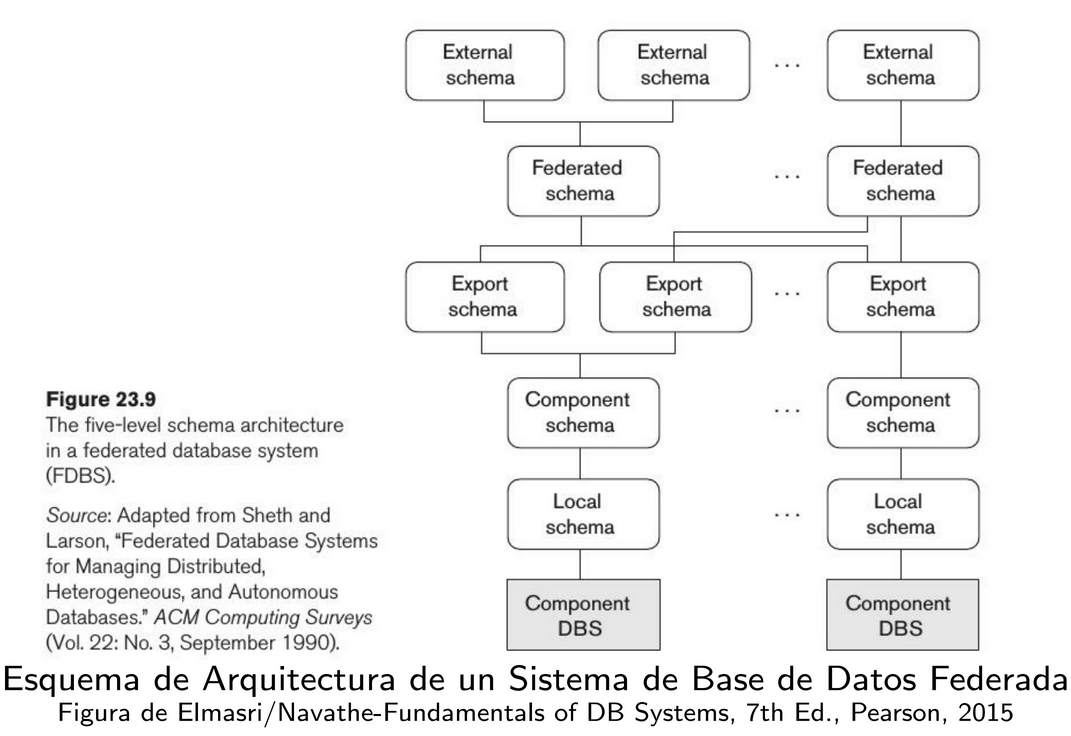
\includegraphics[scale=0.45]{fig/arquitectura-distribuida-federada.png}
\end{figure}




\section*{Datos semi-estructurados y XML}

Los datos estructurados no fueron muy compatibles con el alza de la web, \textbf{HTML}, y otros.

Los datos estructurados tienen un formato estricto, fijo y predefinido pueden relacionarse con otros datos en registros de la misma estructura.

Hacer traducciones constantes de \textbf{HTML} a lenguajes estructurados tiene el problema de volver \textbf{frágil} y propenso a que \textbf{deje de funcionar} los programas, y requerir HTTP requests incluso cuando solo se requiere un valor de una tabla.

Los \textbf{datos semi-estructurados} tienen cierta estructura pero \textbf{no garantizan la predictibilidad y organización} de los \textbf{estructurados}. Aún así, \textbf{los semi-estructurados}, tienen marcas y otros elementos que les permite jerarquizarlos, pero por tanto \textbf{la definición de la estructura esta mezclada con los datos}.

\texttt{XML, eXtensible Markup Language} es un lenguaje parecido a \textbf{HTML} pero no igual, que permite intercambiar datos con cierta estructura \textbf{(semi-estructurado)} como \textbf{JSON} o los \textbf{csv}.
\textbf{Permite representar datos más amigables} para el formato Humano-Computadora, con \textbf{la desventaja} que \textbf{hay mucha redundancia} y \textbf{repetición de los datos a diferencia de los estructurados}.

\textbf{DTD} (Document Type Definition) y \textbf{XML Schema} permiten definir estructuras en \textbf{XML} con el objetivo de asegurar que los archivos \textbf{XML} recibidos o enviados conforman un cierto esquema, \textbf{permiten además chequeos automáticos que verifican que el archivo cumple con dicho esquema}.

\textbf{XPath} es un lenguaje de recuperación y consulta de archivos \textbf{XML}, utiliza jerarquización en base a directorios como una estructura de carpetas.

\textbf{XQuery} es un lenguaje puramente de consultas, que toma conceptos de \textbf{SQL}, \textbf{XQL} y otros lenguajes de consulta para \textbf{XML}.

Además, existen extensiones para \textbf{SQL} que permiten tratar con archivos \textbf{XML} como por ejemplo la extensión de \textbf{Oracle} (y así poder usar \textbf{datos semi-estructurados} en \textbf{entornos estructurados}).
\section*{Mapeo Objeto Relacional (ORM)}
Estos se enfocan en combinar las ventajas de los \textbf{modelos relacionales} (consultas de alto nivel) con los \textbf{orientados a objetos} (tipos de datos complejos como mapas o multimedia). Soportan:
\begin{itemize}
    \item \textbf{Tipos de datos complejos:} Permiten atributos con dominio no atómico para tener un modelo más intuitivo para aplicaciones los manejen. Esto hace que violen \textbf{1FN} aunque mantienen los \textbf{fundamentos matemáticos} de la relación. Algunos de ellos son:
    \begin{itemize}
        \item \textbf{Colecciones o conjuntos:} Particularmente permiten definir \textbf{relaciones anidadas} a través de collect o subconsultas. Soportan \quotes{desanidación}.
        \item \textbf{Estructuras:} Particularmente las definidas por el usuario.
    \end{itemize}
    \item \textbf{Funcionalidades orientadas a objetos:}
    \begin{itemize}
        \item \textbf{Herencia:} Permiten definir tipos en base a otros y los subtipos pueden redefinir métodos de su supertipo (o supertipos con cuidado de no generar conflictos) en su declaración.
        \item \textbf{Referencias:} Apuntan a identificadores de otros objetos y permiten evitar consultas adicionales y juntas a través de expresiones (\textbf{path expressions}).
    \end{itemize}
\end{itemize}
Hay extensiones de SQL que comprenden estas funcionalidades pero no están totalmente implementadas en sistemas actuales (algunas son de uso comercial).
\section*{NoSQL}
Este tipo de bases de datos \textbf{no relacionales} fueron diseñadas a partir de la existencia de datos no estructurados. Se caracterizan por ser \textbf{distribuidas}, de código abierto, y al no tener un esquema definido se basan en el concepto de \textbf{clave/valor}. Aquí almacenan los valores provistos para cada clave y los distribuyen a lo largo de la base. \\
\textbf{Ventajas:}
\begin{itemize}
    \item Suelen tener una interfaz sencilla.
    \item Pueden albergar grandes cantidades de datos con escalamiento horizontal (no tanto vertical).
    \item Pueden recuperar su datos fácilmente gracias a su distribución.
    \item Sus datos pueden ir evolucionando a través del tiempo y convivir con datos de diferentes estructuras.
    \item Consultas que anteriormente eran complejas a través de juntas u otros operadores pueden responderse rápidamente.
\end{itemize}
\textbf{Desventajas:}
\begin{itemize}
    \item No permiten realizar consultas muy complejas.
    \item Su variedad de opciones dificulta saber la más adecuada para cada caso.
    \item Carecen de operaciones de juntas, agrupamiento y ordenamiento.
    \item Su soporte es limitado.
    \item No tienen un lenguaje de consultas definido.
    \item Su administración de transacciones tiene poca garantía.
\end{itemize}

\subsection*{Herramientas y operaciones (todo esto ya no es evaluado en 2022, y fue reemplazado por lo que se ve ahora en Distribuidas (fragmentación y replicación) y en la descripción de NoSQL de Documentos, la cual describe el MapReduce de MongoDB de la forma que es evaluado en 2022).}
\begin{itemize}
    \item \textbf{MapReduce:} Es un marco de trabajo que permite \textbf{procesar paralelamente} grandes volúmenes de datos en varios equipos. Parte de la operación \textbf{Map} que toma los datos de la DB y los transforma en una colección de operaciones que se pueden ejecutar independientemente en diferentes procesadores. A la salida retorna pares \texttt{<clave, valor>} a los que \textbf{Reduce} les aplica la operación asignada y retorna su resultado.
    \item \textbf{Sharding:} Se basa en \textbf{particionar} a los datos de la DB en fragmentos (shards) que se distribuyen a través de servidores. Estos comparten su esquema haciendo que su unión represente la totalidad del dataset. Nótese que esta fragmentación no es trivial y suele hacerse en base al hash de alguno de sus aributos. \\
    \textbf{Ventajas:}
    \begin{itemize}
        \item Permite salvar la imposibilidad de guardar todos los datos en la misma máquina.
        \item Escala horizontalmente.
        \item Brinda tolerancia ante fallas, ya que sólo una porción de los datos quedaría fuera de servicio.
    \end{itemize}
    \textbf{Desventajas:} Ante frecuentes consultas que involucren más de un nodo, su rendimiento decrece.
    \item \textbf{Replicación:} Es el almacenamiento de \textbf{múltiples copias} de la base de datos en diferentes nodos de la red. Puede combinarse con sharding para tener escalabilidad y disponbilidad. Se puede implementar en modo Master-Slave o P2P (Peer to Peer):
    \begin{itemize}
        \item \textbf{Master-Slave:} Este designa a un nodo como \textbf{master} y sobre él efectúa las operaciones de actualización (insert, delete, update), mientras que el resto (\textbf{slaves}) se usan mayormente para lecturas (cada tanto se actualizan). \\
        \textbf{Ventajas:}
        \begin{itemize}
            \item Son ideales para escenarios de muchas lecturas.
            \item En caso de fallar el nodo master, las lecturas pueden continuar en los slaves y se los puede configurar para que lo reemplacen.
        \end{itemize}
        \textbf{Desventajas:}
        \begin{itemize}
            \item El nodo master puede representar un cuello de botella para las escrituras.
            \item Las lecturas pueden ser inconsistentes según la frecuencia en que se actualice cada réplica. Para ello puede implementarse un sistema en el que un valor se considere consistente al estar en la mayoría de los nodos, pero este requiere de una comunicación más rápida y confiable entre ellos.
        \end{itemize}
        \item \textbf{Peer to Peer (P2P):} Aquí todos los nodos (\textbf{peers}) poseen el mismo nivel de jerarquía y pueden manejar tanto lecturas como escrituras. \\
        \textbf{Ventajas:}
        \begin{itemize}
            \item Evitan los cuellos de botella al tener un sistema descentralizado y tienen mayor tolerancia a las fallas.
            \item El rendimiento es potencialmente mayor ya que todos los nodos son capaces de responder a las peticiones.
        \end{itemize}
        \textbf{Desventajas:} Las lecturas pueden ser inconsistentes y las escrituras, conflictivas. Tenemos dos posibles estrategias para tratar estos problemas:
        \begin{itemize}
            \item \textbf{Concurrencia pesimista:} Uso de locks que asegure la consistencia y prevenga conflictos a pesar de ir en contra de la disponibilidad.
            \item \textbf{Concurrencia optimista:} No uso de locks, lo cual puede generar inconstencias basándose en la propagación de los valores hasta llegar a un estado consistente. Para asegurarse de que no sucedan suele  combinarse con un sistema de votación parecido a master-slave.
        \end{itemize}
    \end{itemize}
\end{itemize}

\hypertarget{oltp}{}
\subsection*{OLTP} 
Es un tipo de procesamiento de Datos. En la mayoría de los casos que vimos (\textbf{Relacionales}) y verémos a continuación de tipos de DBMS, se piensa en modelos de procesamiento de \textbf{On Line Transactional Processing} (no obstante, algunos DBMS \textbf{NoSQL}, están pensados para un uso \textbf{OLAP} o mixto \textbf{OLTP/OLAP}). Están pensadas para las bases de datos que deben soportar la ``operación'', el ``día a día''. Buscan poder resolver muchas transacciones que puedan seleccionar, insertar y modificar datos eficientemente (a grandes rasgos).

\hypertarget{olap}{}
\subsection*{OLAP}
\textbf{On Line Analitical Processing} 
es otro tipo de procesamiento de datos, dónde las Bases de Datos que cumplen con tener un tipo de procesamiento de datos \textbf{OLAP}, buscan hacer análisis estadístico, con datos sumarizados, de acceso poco frecuente, desnormalizados, por columna para cálculos estadísticos rápidos y eficientes. Ejemplos de esto son las Bases de Datos \textbf{Column Store} (notar que no son lo mismo que las \textbf{Column Family}).

\subsection*{Tipos de bases NoSQL}
Los tipos de bases NoSQL más comunmente usados son los basados en: key-value pair (pares clave-valor), document (documentos), column family (grupos de columnas) e graph (grafos).

Se estima que las bases de datos Key-value son las que son capaces de almacenar los volúmenes mayores de datos, seguidas de las ColumnFamily, las de Documentos, las de grafos, y finalmente las SQL.

No obstante la complejidad de los datos modelables por bases de datos de Grafos, es mayor a la de documentos, seguida de las de Column Family, y las Clave-valor tienen mucha dificultad para modelar relaciones complejas de los datos.

\subsubsection*{Key-value pair databases}
Es la más sencilla ya que guarda cada ítem como una \textbf{clave asociada a un valor} (como un diccionario). Las claves deben ser \textbf{únicas} dentro del dominio manejado para identificar al ítem unívocamente (para esto se pueden tener namespaces y/o buckets). \\
Los datos guardados constituyen su información y no tienen un esquema definido, por lo que \textbf{no tienen restricciones} en cuanto a tamaño ni tipo: texto plano, XML, JSON, imagen, etc. Esto no salva que pueda haber datos redundantes y no implementan integridad referencial. \\
\textbf{Ventajas:}
\begin{itemize}
    \item Su escalabilidad hace que se adecúen a la nube, servicios en la web y aplicaciones móviles, ya que no es necesario consultar todas sus entradas para obtener un valor.
    \item Permiten almacenar objetos variados al asociarlos a claves. Esto las hace útiles para el código orientado a objetos.
\end{itemize}
\textbf{Desventajas:}
\begin{itemize}
    \item La integridad de los datos y sus restricciones deben ser manejadas por los programadores.
    \item La falta de estructura limita el análisis posible que pueda efectuarse sobre los datos.
    \item Su enfoque en la escalabilidad limita su funcionalidad y complejidad.
\end{itemize}

\subsubsection*{Document databases}
Se asemejan a las anteriores pero guardan sus datos en base a \textbf{documentos} (strings o representaciones binarias de strings). Estos pueden diferir en su estructura (semi-estrcuturados, JSON, XML) y pueden contener listas de atributos e incluso \textbf{documentos embebidos}. Entre sus datos pueden contener metadata con índices para referirse a sus campos. \\
Suelen manejarse a través de motores de DB como \textbf{MongoDB}. Este tiene escala horizontal gracias al sharding y replicas. Además en su API tiene incorporadas las funcionalidades de MapReduce para procesamiento batch (procesar y resumir grandes volúmenes de datos) y sabe operar con agregaciones como SQL. Permite además implementar búsquedas ad-hoc por campos y rangos particulares. Otros motores incluyen RavenDB, RethinkDB y CouchDB. \\
\textbf{Ventajas:}
\begin{itemize}
    \item Los documentos pueden representar flexiblemente entidades, ya que no requieren la definición de sus atributos previamente.
    \item Su información es accesible a través de lenguajes de consultas y APIs dedicados, a diferencia de key-value donde es necesario acceder a la clave previamente.
    \item La incrustación de documentos evita implementar juntas en las consultas, mejorando el rendimiento. Esta pueden especificarse a través de su esquema lógico dado por su \textbf{diagrama de interrelación de documentos (DID)}.
\end{itemize}
\textbf{Desventajas:} La flexibilidad de la información que maneja puede acomplejizar la interpretación de los datos en un programa.

\subsubsection*{Column family databases}
Almacenan sus datos en \textbf{columnas} que asocian un nombre con un valor. Estas se agrupan en \textbf{filas} (row) y las que suelen accederse simultáneamente en las consultas se agrupan en \textbf{familias} (column families). No requieren predefinir un esquema para agregar columnas nuevas. Además, tienen mecanismos naturales de partición vertical y su almacenamiento es multi-dimensional (mapas o vectores asociativos). \\
Superficialmente se asemejan a las \textbf{bases de datos relacionales}, pero con algunas diferencias:
\begin{itemize}
    \item No implementan juntas ya que su set de columnas no está predefinido.
    \item Suelen estar denormalizadas de manera de poder guardar en una fila toda la información relacionada con una entidad particular.
\end{itemize}
\textbf{Ventajas:}
\begin{itemize}
    \item Permiten replicar y distribuir sus datos fácilmente en múltiples nodos de la red.
    \item Tienen un modelo de fácil acceso a través de lenguajes de consulta parecidos a SQL.
    \item Las column families favorecen el rendimiento de las consultas de agrupamiento (máximo, mínimo, promedio, etc.).
    \item Su escalabilidad ser ve favorecida al permitir que no todas las columnas tengan valores asociados.
    \item Pueden usar timestamps para almacenar diferentes versiones de un valor en el tiempo.
\end{itemize}
\textbf{Desventajas:} 
\begin{itemize}
    \item No son adecuadas para datos relacionales.
    \item No proveen consistencia inmediata (son BASE).
\end{itemize}

\subsubsection*{Graph databases}
Estas almacenan sus datos como \textbf{nodos} conectados a través de \textbf{relaciones dirigidas}. Ambas estructuras pueden contener información compleja. SQL Server y Oracle agregaron funcionalidad basada en ellas. \\
\textbf{Ventajas:}\
\begin{itemize}
    \item Ejemplos como \textbf{NEO4J} cumplen con garantías \textbf{ACID}, a diferencia de muchas otras opciones NoSQL.
    \item Permiten almacenar relaciones y manejarlas eficientemente al pensar a cada nodo como una entidad.
    \item Se adecúan a los problemas enfocados en relaciones y basados en \textbf{grafos} (redes sociales, conexiones, recorridos, etc.) que en las bases relacionales tendrían el costo de muchas juntas y consultas.
    \item En el caso de \textbf{NEO4J}, este incluye capacidades para sharding (fragmentación) y replicación. La replicación usa un sistema de nodos \textbf{``Core''} y nodos \textbf{``Read Replica''}. Una escritura es confirmada cuando todos los servidores Core la confirman. Por tanto da posibilidades de escalabilidad y alta disponibilidad.
\end{itemize}
\section*{Otras bases de datos}
\subsection*{Stream databases}
Son bases utilizadas para situaciones en que \textbf{los datos se cargan continuamente} (páginas web, sensores, trayectorias de paquetes). Se manejan a través de un \textbf{DSMS} que al recibir las consultas responde respecto de los datos que van ingresando y están disponibles por un período corto de tiempo. Aquí el \textbf{stream} es un conjunto de pares \texttt{<s, t>} donde $s$ es una tupla y $t$ un timestamp con su tiempo de llegada. \\
Para contemplar la \textbf{validez} de los datos en las consultas se impone una restricción sobre la parte del stream a procesar. Esta es la \textbf{ventana} y se puede expresar diferente según la implementación del lenguaje:
\begin{itemize}
    \item \textbf{Landmark:} Mantiene fija la parte más antigua y la más nueva avanza conforme llegan tuplas al stream.
    \item \textbf{Sliding:} Ambos extremos de la tupla van avanzando a medida que llegan tuplas nuevas.
\end{itemize}

\subsection*{Spatial databases}
Se enfocan en los \textbf{Tipos de Datos Espaciales} \textbf{(SDT: Spatial Data Types)}, como puntos, líneas, polígonos, etc. Proporcionan indexación espacial y algoritmos eficientes de unión espacial y distancias entre cualquier tipo de par de \textbf{SDTs} usados. Comprenden a las \textbf{bases de datos geográficas}. Sus consultas suelen incluir:
\begin{itemize}
    \item Objetos de un cierto tipo en cierto rango.
    \item Vecino más cercano de un cierto tipo de objeto.
    \item Intersección o superposición entre 2 objetos.
\end{itemize}
\textbf{PostGIS} es un ejemplo de una extensión, que convierte a \textbf{PostgreSQL} en una Base de Datos Espacial. Por tanto responde queries \textbf{SQL}, es \textbf{ACID}, y resuelve los problemas antes mencionados.

\subsection*{Cloud DataBases (CDBs)}

Las Cloud Data Base Management Systems (CDBMSs) son DBMSs distribuidas que proveen todo el paquete incluyendo el poder de computo accesible como un servicio desde internet, es por esto y dado que no se almacenan in situ como otras DBMSs que los datos se  guardan  encriptados. Se paga por tiempo, espacio físico y poder de computo. Hay versiones relacionales y no relacionales.

\textbf{Ventajas:}\
\begin{itemize}
    \item Muy fáciles de escalar, generalmente solo implica solicitar una mejora del servicio obtenido.
    \item Reduce el costo de tener un DBMS, especialmente para pequeños y medianos usuarios. Para grandes usuarios a largo plazo dependerá de más factores.
    \item La tolerancia a fallas tiende a ser de muy alta calidad y a veces personalizable.
\end{itemize}

\textbf{Desventajas:}\
\begin{itemize}
    \item La seguridad puede ser buena pero fuera de nuestro alcance garantizarla.
    \item Hay dependencias legales en los datos que pueden impedirnos usar CDBMSs para ciertos datos.
\end{itemize}

\subsection*{Multi Tenant DataBases}

Si bien no es un tipo de Base de Datos por si misma, es un concepto que puede definir algunas Bases de Datos, especialmente en los modelos de Bases de Datos como un Servicio (DBaaS).

Puede tratarse de una Base de Datos por cliente, con algún recurso compartido (Database-per-tenant/Multi-Database). Una Base de Datos para varios o todos los clientes, pero separadas por schemas distintos para cada uno (Multi-Schema). O un único schema global que es usado por todos los clientes en la misma Base de Datos compartida (Shared-Schema).

\subsection*{In-memory databases}
Son bases de datos \textbf{cargadas completamente en memoria}. Existen de dos tipos:
\begin{itemize}
    \item \textbf{Sin persistencia:} Un corte en el suministro de energía hace que se pierda toda la base (ej: MemBase).
    \item \textbf{Con persistencia} (ej: Redis, Sap Hanna).
\end{itemize}
Aquí todas la interacciones con la base se resuelven en memoria y se \textbf{escribe continuamente al log}, aprovechando que es secuencial para que las escrituras físicas sean rápidas. \\
Pueden almacenarse por \textbf{filas} o por \textbf{columnas}. Las primeras son útiles para operaciones de selección mientras que las otras para proyección y ocupan menos espacio.

\textbf{Volt DB} es un ejemplo de \textbf{IMDB} que cumple \textbf{ACID}, responde a queries escritas en \textbf{SQL}, y asegura durabilidad a través de command logging y replicas.

\textbf{Redis} también es una \textbf{IMDB} con servicio de servidor (Master) y cliente (Slave). Es útil porque funciona también como Base de Datos de Streams y de datos Geoespaciales, y puede observar cambios de un valor por medio de un comando \texttt{WATCH}.

\subsection*{Column Store databases}
\textbf{No confundir} con las \textbf{Bases de Datos Column Family}. Las \textbf{Bases de Datos Column Store} pueden ser Bases de Datos Relacionales como las SQL convencionales, con la diferencia que guardan los contenidos de las tablas por columna y no por fila. Esto las hace mucho más adecuadas para procesamientos analíticos como los procesamientos \textbf{OLAP} (ya que operaciones analíticas como agregaciones que requieren pocas columnas son mucho más eficientes (proyecciones mucho más baratas), pero a costa de que los procesos \textbf{OLTP} sean más costosos (selecciones, y en particular modificaciones e inserciones en tablas son muchísimo más costosas).

\textbf{Vertica Database} es un ejemplo de CSDB que cumple \textbf{ACID} y responde a queries escritas en \textbf{SQL}.

\subsection*{Resorce Description Format (RDF) management systems}
Comprende los datos \textbf{explícitamente declarados} y los \textbf{implícitos} generados a través de \textbf{restricciones semánticas} (reglas de entailment). Las consultas entonces se pueden resolver convirtiendo todos los datos en explícitos o reescribiendo la consulta de manera que contenga las expansiones (a través de reglas). Ejemplo:

\begin{center}
    \ttfamily
    \begin{tabular}{c|c}
        Explícito & Implícito \\
        a) Sócrates es humano & Sócrates es mortal \\
        b) Los humanos son mortales
    \end{tabular}
\end{center}

\subsection*{Mobile databases (Opcional, no evaluado en 2022)}
Son las enfocadas en el creciente uso de \textbf{dispositivos móviles}, ya que pueden instalarse en uno a través de una red móvil. Aquí el cliente y el servidor se conectan de forma \textbf{inalámbrica} y la memoria caché se usa para almacenar datos frecuentes y transacciones para que no se pierdan por un fallo de conexión. \\
Sus aplicaciones se clasifican en:
\begin{itemize}
    \item \textbf{Verticales:} Los usuarios pueden acceden a los datos en una celda específica y fuera de ella la información no está disponible (sistema de plazas libres en un estacionamiento).
    \item \textbf{Horiontales:} Los datos se distribuyen por todo el sistema y los usuarios pueden acceder a ellos desde cualquier celda (acceso al correo electrónico).
\end{itemize}
Los DBMS móviles deben además proveer la capacidad de:
\begin{itemize}
    \item Comunicarse con el servidor centralizado de la DB a través de comunicación inalámbrica o acceso a Internet.
    \item Replicar y sincronizar los datos en el servidor centralizado y el dispositivo móvil.
    \item Responder a una consulta de acuerdo con la \textbf{localización} del dispositivo móvil (ya sea, el lugar del que se efectuó la consulta, el lugar donde terminó o el indicado por ella). La movilidad de las estaciones de acceso puede dificultar la optimización por el coste de comunicación involucrado (más aún si los datos residen en una estación móvil). A esto se le suma la variabilidad del ancho de banda.
\end{itemize}
Si bien la tecnología móvil puede ser de gran provecho para negocios y empresas por optimizar la productividad, racionalizar las operaciones y crear nuevas fuentes de ingreso, los datos accesibles de manera remota pueden ser críticos a la corporación. Por ende, su \textbf{estrategia de seguridad} debe contemplar las maneras de gestionar y garantizar su seguridad en cualquier sitio y hora. Para ello se aplica la \textbf{autentificación de usuarios} cada vez que se quiera acceder a una nueva capa de confidencialidad y funcionalidad de los sistemas corporativos. De no estar autorizado, el acceso debe ser denegado.
\section*{Big Data}

Big Data se los define a los datos que cumplen con las \textbf{5 V's} en mayor o menor medida.

\begin{itemize}
    \item \textbf{Volumen:} presentan un gran \textbf{volúmen} de datos.
    \item \textbf{Velocidad:} accesibles a \textbf{velocidades} que permiten el acceso en cuestión de milisegundos (cómo es el caso de los mercados bursátiles).
    \item \textbf{Variedad:} con datos de gran \textbf{variedad}, de muchos entornos distintos y diversos, que pueden estar estructurados o no, venir de paradigmas varios, e integrar muchos modelos.
    \item \textbf{Veracidad:} donde los datos pueden ser poco confiables, ruidosos, mezclar orígenes de datos que al combinarlos, su output puede generar incertidumbre, y que por tanto es necesario tratarlos, analizarlos, categorizarlos según fiabilidad, con el fin de poder corroborar con algún criterio su \textbf{Veracidad}.
    \item \textbf{Valor:} teniendo en cuenta que los datos proveen valor intrínseco al permitir tomar decisiones eficientes y precisas que le otorgan \textbf{Valor}.
\end{itemize}
\section*{OpenData}
Es un \textbf{movimiento} que apoya la \textbf{difusión de los datos} por parte de los Estados, organismos internacionales y empresas para promover su análisis y utilización en \textbf{formatos abiertos} para crear visualizaciones, aplicaciones y herramientas. \\
Los datos son publicados con dos motivos principales:
\begin{itemize}
    \item Transparencia y participación ciudadana (open goverment, repercutió en América Latina)
    \item Generación de servicios para empresas y de valor para iniciativas privadas (repercutió en Europa)
\end{itemize}
Las publicaciones son públicas o semi-públicas y son accedidas por parte del periodismo, ongs, emprendedores y entidades académicas o estudiantiles. El acceso se considera \textbf{abierto} si al estar a disposición del público los datos cumplen con los siguientes principios:
\begin{enumerate}[label=\roman*]
    \item \textbf{Completo:} Todos están disponibles, sin limitaciones de seguridad o privilegio.
    \item \textbf{De primera fuente:} Son coleccionados desde la fuente, con el mayor grado posible de granularidad, sin ningún tipo de modificación o agregación.
    \item \textbf{En tiempo:} Están disponibles tan pronto como sea necesario para preservar su valor.
    \item \textbf{Accesible:} Están disponibles para el rango más amplio de usuarios y propósitos.
    \item \textbf{Procesables por computadoras:} Están estructurados razonablemente como para permitir su procesamiento automático.
    \item \textbf{No discriminatorios:} Están disponibles para todos, sin necesidad de registro (pueden ser accedidos de forma anónima, incluso a través de proxies anónimos).
    \item \textbf{No propietario:} Tienen que tener un formato del que ninguna entidad tenga control exclusivo.
    \item \textbf{Sin licencia:} No deben estar sujetos a derechos de autor, patente, etc.
\end{enumerate}

\section*{Administración de datos}
\subsection*{Calidad de datos}
Los \textbf{datos registrados} en una base pueden ser de varios tipos:
\begin{itemize}
    \item \textbf{Registros:} Cada valor es un registro y se puede almacenar en una \textbf{matriz} (como conjunto fijo de atributos), \textbf{documento} (vector de términos de significado ámplio) o ser parte de una \textbf{transacción} (involucrando a un conjunto de ítems).
    \item \textbf{Semi-estructurados:} Representados a través de \textbf{XML} (lenguaje de marcación jeráquico muy utilizado para el intercambio de información) o \textbf{JSON} (similar al anterior pero con otras funcionalidades).
    \item \textbf{Grafos:} Enfocados en problemas basados en grafos o redes.
    \item \textbf{Ordenados:} Su criterio de orden puede depender de una secuencia, el espacio o el tiempo (\textbf{stream:} cuando estos fluyen continuamente con diferentes velocidades).
\end{itemize}
Ahora, teniendo los datos guardados suele presuponerse que estos son \textbf{correctos} o que su \textbf{validez} es eterna. La \textbf{calidad de datos} nos dice que es necesario \textbf{monitorearlos permanentemente}, con dinero y/o esfuerzo para que eso pase. Sobre esto es que residen una serie de posibles errores en los datos:
\begin{itemize}
    \item Fuera de rango
    \item Falta de estándar
    \item Invalidez
    \item Diferencias culturales
    \item Discrepancias en el formato
    \item Cosméticas
    \item Inconsistencias provenientes de metadata
    \item ...
\end{itemize}
Para analizar la calidad tenemos varias opciones:
\begin{itemize}
    \item \textbf{Análisis univariado:} Obtener el valor mínimo, máximo, media, mediana, moda, histogramas y demás datos estadísticos de cada variable.
    \item \textbf{Análisis bivariado:} Obtener el coeficiente de correlación, tablas de contingencia, diagramas de dispersión y demás entre pares de variables.
    \item \textbf{Perfilado de los datos:} Analizar la información en cada sitio y buscar inconsistencias.
\end{itemize}

\subsection*{Gobierno de datos}
\textbf{Definición:} Según la DAMA (Data Management Association) y la Data Resource Management, es el \quotes{\textit{desarrollo y ejecución de arquitecturas, prácticas y procedimientos que manejan adecuadamente las necesidades del ciclo de vida de datos de una empresa}}. Esto incluye aspectos de calidad, arquitectura, seguridad y metadata de los datos y comprende a \textbf{toda la organización}, no sólo al sistema en sí por ser los datos un \textbf{activo} de ella. \\
En su implementación conviene empezar con un objetivo poco ambicioso para mostrar su utilidad y luego ir incrementando su \textbf{nivel de madurez}. Nótese que puede necesitarse apoyo económico. \\
\textbf{Nivel de madurez:} \\
El nivel de madurez del gobierno de datos se divide en:
\begin{itemize}
    \item \textbf{Indisciplinado:} Las decisiones de negocio dependen de la tecnología, los datos pueden ser inconsistentes o duplicados y hay poca flexibilidad para mantener los cambios de negocio.
    \item \textbf{Reactivo:} El negocio influye sobre las decisiones de tecnología, la información es redundante y poco controlada y hay un alto costo en mantener múltiples aplicaciones.
    \item \textbf{Proactivo:} Los equipos de negocio y tecnología trabajan de manera colaborativa y los datos son un activo de la compañía.
    \item \textbf{Gobernado:} Los modelos de negocio definen las decisiones tecnológicas, hay procesos estandarizados para definir la gestión de los activos de los datos, las decisiones corporativas se toman con datos certeros y se obtienen beneficios por la aplicación del programa de gobierno.
\end{itemize}
\textbf{Roles principales:} \\
Hay una serie de roles involucrados en el gobierno de datos:
\begin{itemize}
    \item \textbf{Chief Data Officer:} Máximo responsable del programa y lider del equipo. Encargado de definir y/o colaborar en las iniciativas del gobierno de datos, promoviendo, negociando y justificando cambios en la estrategia de datos corporativa.
    \item \textbf{Arquitecto de datos:} Desarrollador de la arquitectura de datos para atender a los requerimientos de negocio. Encargado de desarrollar estándares y procedimientos de diseño y modelado, supervisarlos para cada componente y aprobar las características de desarrollo de aplicaciones e interfaces que afecten la arquitectura.
    \item \textbf{Data owner:} Máxima autoridad de aprobación respecto de los riesgos de gobierno en su dominio. Gestiona el ciclo de vida de los datos con sus permisos de acceso, calidad y riesgos, colabora en el gobierno de datos y conoce su significado.
    \item \textbf{Data steward:} Quienes apoyan a los anteriores al comprender sus procesos de negocio y datos producidos. Responsables de escribir e implementar reglas de calidad de datos, atender a sus problemas y escalarlos de darse el caso. Tiene responsabilidades concretas y puede efectuar acciones en nombre del dueño para liberar el flujo.
    \item \textbf{Custodio de datos:} Soporte en las áreas de bajo nivel y de telecomunicaciones de las plataformas, sistemas y aplicaciones en que residen los datos de los anteriores. Pueden tener cierta responsabilidad operativa y se encargan de mantener la integridad y seguridad de los datos, cumpliendo con las políticas del programa.
\end{itemize}

\begin{figure}[H]
    \centering
    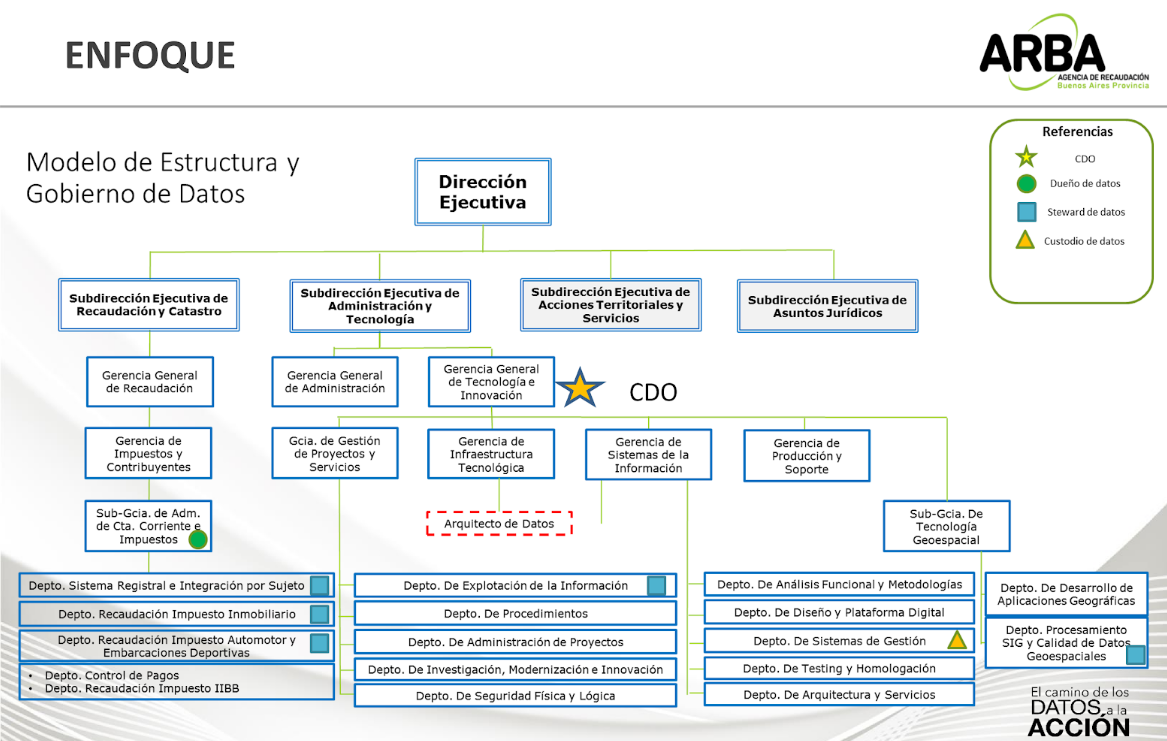
\includegraphics[scale=0.4]{fig/modelo-gobierno-de-datos.png}
\end{figure}

\subsection*{Administrador de datos}
Es una persona (o conjunto de ellas) responsable de \textbf{administrar} los datos de manera \textbf{funcional o lógica}. Se diferencia del \textbf{DBA} en que el segundo es \textbf{especialista} en el motor de la DB. \\
Sus tareas principales son:
\begin{itemize}
    \item Recolectar y analizar los requerimientos, modelando el negocio en base a ellos (conceptual y lógico).
    \item Definir estándares sobre los datos y asegurar su cumplimiento.
    \item Conducir sesiones de definición de datos.
    \item Manejar y administrar repositorios de metadata y herramientas de modelado.
    \item Asistir al DBA en la creación de modelos físicos a partir de los lógicos.
\end{itemize}
Nótese que la \textbf{definición de los datos} suele encontrarse en dos lugares desde el punto de vista del negocio:
\begin{itemize}
    \item \textbf{La mente de las personas:} Si son reglas no escritas existentes en todas las áreas que interactúan con ellos. Estas son vulnerables a baja calidad por falta de consistencia o confianza.
    \item {Los modelos de los datos:} Se representan a través de las herramientas de modelado pero suelen reflejar sólo el estado final y no los cambios.
\end{itemize}

\subsection*{Privacidad}
Es una preocupación creciente con numerosas \textbf{regulaciones} locales e internacionales al respecto. Se centra en garantizar la \textbf{protección de los datos} para todos sus usuarios más allá de dónde estén. En el ámbito local (Argentina) existen numerosos secretos estadísticos, fiscales y educativos, más allá de haber una agencia de acceso a la información pública y una dirección nacional de protección de datos personales.

\section*{Arquitectura de Datos}

La arquitectura de datos es un conjunto de especificaciones que ayudan en la estandarización de como una organización recibe, almacena, transforma, distribuye y usa los datos. Esto ayuda en las "inversiones en datos".

\subsection*{Características de una Buena Arquitectura de Datos}

Una buena arquitectura de datos debe ser:

\begin{itemize}
    \item \textbf{Colaborativa:} todas las áreas deben colaborar.
    \item \textbf{Administrada:} Buena gobernanza.
    \item \textbf{Simple:} Disminuir variedad de herramientas usadas, duplicación de datos, y facilitar su modos de uso.
    \item \textbf{Elástica:} Poder manejar demandas crecientes y cambiantes de su uso.
    \item \textbf{Segura:} Buenas políticas de seguridad.
    \item \textbf{Resiliente:} que tenga alta disponibilidad y capacidad de recuperación ante fallas.
\end{itemize}
\textbf{}

\subsection*{Data as a Service (DaaS)}

\textbf{Data as a Service (DaaS)} es una estrategia de administración de datos en la que una compañía renta su capacidad de almacenamiento, integración, procesamiento y servicios de analítica a otras compañías o terceros a través de un servicio en la nube.

\subsection*{Integraciones de Bases de Datos}

Las bases de datos pueden ser integradas unas a otras por razones como fusiones de compañías o federaciones. Herramientas para facilitar el proceso pueden  seguir estrategias:

\textbf{ETL:} Extraction - Transform - Load

\textbf{ELT:} Extraction - Load - Transform

La fase que se haga  segunda tiene prioridad por sobre la tercera. 

\textbf{ETL} transforma los datos en una staging area antes de cargarlo a la Data Warehouse donde se  almacenará para su análisis.

\textbf{ELT} en cambio, lo carga y transforma en la misma Data Warehouse, haciéndose allí su futuro análisis, permitiendo usar el resultado y transformarlo nuevamente en el futuro sin requerir nuevas cargas, pero cualquier carga de datos nuevos va a requerir una nueva transformación.

\subsection*{Federaciones y Fusiones como arquitectura de Datos}

\textbf{Las Federaciones} construyen un esquema virtual global que sabe consultar con mapeos predefinidos a cada base de datos integrada a la Federación, y con ello responde las queries que se le indiquen. No obstante no guarda ningún dato. Es útil para consultas a Bases de Datos diversas que fueron desarrolladas de formas distintas y que necesitan cooperar para un mismo fin, como por ejemplo, una federación de aerolíneas que quiere publicar los vuelos de muchas aerolíneas (despegar.com), o una federación de hoteles que desea publicar la disponibilidad de distintos hoteles con distintas Bases de Datos (hoteles.com).

En cambio \textbf{las fusiones o adquisiciones} de compañías tienden a definir mapeos que transforman los datos de la compañía adquirida generalmente a la estructura de la compañía que la adquirió, la cual además alojará copia de dicho datos transformados a la  estructura de la compañía que realizó la adquisición.
\section*{Data Mining}

Es la \textbf{extracción} de patrones o \textbf{información interesante}, es decir, no trivial, implícita, previamente desconocida y potencialmente útil, de grandes bases de datos (como data warehouses). Su resultado es \textbf{el KDD} (Knowledge Discovery in Databases o Descubrimiento de Conocimiento en Bases de Datos).

\subsubsection*{Outliers}
Es importante tener datos de Calidad para estos algoritmos, y el tratamiento de outliers es muy importante.
Dentro del conjunto de datos analizado los outliers siguen un comportamiento diferente al resto en una o más variables. Si bien se los puede usar para \textbf{detectar anormalidades}, generalmente pueden ensuciar o influir en nuestros resultados y conviene descartarlos. Esta \textbf{variación} puede provenir de:
\begin{itemize}
    \item \textbf{La fuente:} Surge de las observaciones y se la considera un \textbf{comportamiento natural} en relación a cierta variable de estudio.
    \item \textbf{El medio:} Surge del mal uso de la técnica para medir una variable o cuando no exista una valoración exacta de ella. Comprende los \textbf{redondeos forzosos} en variables continuas.
    \item \textbf{El experimentador:} Se clasifican en:
    \begin{itemize}
        \item \textbf{Error de planificación:} Cuando no se delimita correctamente la población o se realizan observaciones de otra.
        \item \textbf{Error de realización:} Se valora incorrectamente a los elementos (transcripciones erróneas, falsas lecturas con los instrumentos de medición, etc.).
    \end{itemize}
\end{itemize}
De allí se dice que una \textbf{observación atípica} surge de primer tipo de variación, mientras que una \textbf{errónea} de los otros dos. Ambas pueden ser outliers y es conveniente estudiarlas antes de eliminarlas.

Otro concepto importante es la estimación de la precisión del modelo. Para ello se debe construir un conjunto de datos de entrenamiento, y otro distinto e independiente de testing. La independencia evita potenciales overfittings.

La precisión del modelo dependerá de los resultados en el conjunto de test, con el  cual  se  puede construir una matriz de confusión, dividiendo los resultados en correctos (la diagonal de la matriz), falsos positivos, y falsos negativos para problemas de decisión binaria.

\subsubsection*{Funcionalidades del Data Mining}

Entre sus funcionalidades tenemos:
\begin{itemize}
    \item \textbf{Descripción de conceptos:} Caracterizar y discriminar a los datos a través de sus características (generalizar, resumir, contrastar).
    \item \textbf{Asociación:} Establecer una relación de correlación y causalidad.
    \item \textbf{Clasificación y predicción:} Encontrar modelos o funciones que describan y distingan clases para futuras predicciones. Estos se pueden presentar de varias maneras (árboles de clasificación, reglas, redes neuronales) y nos permiten predecir valores faltantes.
    \item \textbf{Cluster analisis:} Agrupar los datos en clases maximizando su similitud y minimizándola entre clases.
    \item \textbf{Análisis de outliers:} Detectar y comprender aquellos datos que no respetan el comportamiento general.
    \item \textbf{Análisis de tendencias y evolución:} Comprender la regresión, patrones secuenciales y similitudes a través del tiempo.
\end{itemize}
Para ello se tiene una serie de técnicas que pueden ser:
\begin{itemize}
    \item \textbf{Supervisadas:} Se basan en un conjunto de entrenamiento con sus respuestas anotadas (redes neuronales, árboles de decisión, regresión).
    \item \textbf{No supervisadas:} Deben inferir una función para describir una estructura oculta a partir de datos no etiquetados (clustering, reglas de asociación).
\end{itemize}

\subsection*{Redes neuronales artificiales (RNA)}
\textbf{Definición:} Son sistemas capaces de \textbf{aprender de sus propios errores} y adaptarse a condiciones variantes y ruido para predecir un estado futuro al asociar entradas a respuestas. Se usan para resolver problemas a \textbf{gran escala} (asociación, evaluación y reconocimiento de patrones) o \textbf{difíciles de calcular} (aproximadamente con respuestas rápidas y buenas). \\
\textbf{Características:}
\begin{itemize}
    \item Aunque no se propagan siguiendo una secuencia predefinida de instrucciones, sólo resuelven \textbf{problemas resolvibles} por el cerebro humano.
    \item Se procesan paralelamente a través de un gran número de elementos \textbf{altamente interconectados} entre sí.
    \item Pueden mejorar su rendimiento al combinarse con otras herramientas (lógica difusa, algoritmos genéticos, sistemas expertos, estadísticas, transformada de Fourier, wavelets).
    \item No son útiles para cálculos precisos, procesamiento serie ni reconocer algo que no siga algún tipo de \textbf{patrón}.
    \item Se basan en modelos simplificados de neuronas reales (modelan el axón, las dendritas, la sinápsis y el cuerpo de la célula).
\end{itemize}
\textbf{Entrenamiento:} \\
El entrenamiento de una RNA sigue una \textbf{regla delta generalizada} consistente en un proceso con todos los datos de entrenamiento que puede repetirse varias veces:
\begin{enumerate}
    \item Calcular la diferencia entre la salida resultante y la esperada.
    \item Corregir los valores de las entradas para achicar las diferencias en base a una constante \textbf{delta} muy pequeña.
\end{enumerate}
De esa forma se busca que la diferencia se vaya minimizando \textbf{de a poco}, ya que de hacerlo de golpe se puede modificar demasiado lo aprendido anteriormente. \\
\textbf{Tipos:} \\
Entre los tipos de RNAs más utilizados tenemos:

\begin{itemize}
    \item Redes Neuronales Profundas es un termino paraguas para muchos tipos de Redes Neuronales pero que poseen muchas capas, dándole gran profundidad a muchas de ellas. Su principal problema es el gran costo computacional que implica entrenarlas debido a la gran cantidad de nodos que requieren entrenarse/optimizarse, y todas las conexiones que poseen.
    \item Las Redes Neuronales de Convoluciones son más sencillas, basadas en la operación matemática de la convolución. Buscan percibir  detalles de más alto nivel, y generalmente se usan para detección de patrones en imágenes como por  ejemplo bordes.
\end{itemize}

Redes neuronales que no aparecen en las diapositivas de 2022:

\begin{itemize}
    \item Perceptrón multicapa
    \item Red de Hopfield (mapas asociativos)
    \item \textbf{Red de Konohen (SOM, mapas auto-organizativos):} Se basan en evidencias de cómo las neuronas del cerebro organizan su información, y en ellas la actualización delta sólo se realiza en la neurona cuyos pesos tengan la distancia mínimo con el valor a entrenar, afectando en menor medida a sus vecinas.
\end{itemize}

\subsection*{Árboles de decisión}
\textbf{Definición:} Son modelos en forma de árbol que se utilizan para \textbf{clasificar} una entrada desconocida según sus \textbf{atributos}. Se componen de nodos internos con preguntas condicionales y entendibles sobre ellos, y hojas con su etiqueta o clase a predecir. \\
\textbf{Construcción:} \\
Para construirlo se parte de todos los ejemplos de la raíz del árbol y se los va dividiendo recursivamente a través de los atributos elegidos. Seguidamente, se podan las ramas con outliers o ruido (\textbf{prunning}). \\
Considerando que el modelo se construye en base a clases existentes de entrenamiento, de este se obtienen las \textbf{reglas de clasificación}. De allí, para estimar su \textbf{precisión} se debe aplicarlo sobre un conjunto de prueba y comparar sus resultados con los reales, tomando el porcentaje correctamente clasificado. \\
\textbf{Prunning:} \\
En el prunning entra en juego el \textbf{overfitting} basado en adaptar el árbol demasiado al conjunto de entrenamiento y puede mediarse a través de:
\begin{itemize}
    \item \textbf{Preprunning:} Interrumpir la construcción de un nuevo nodo si la mejora está por debajo de cierto umbral (difícil de definir).
    \item \textbf{Postprunning:} Quitar ramas de un árbol ya construido (usando otro conjunto de entrenamiento, por ejemplo).
\end{itemize}

\textbf{Ventajas:}

\begin{itemize}
    \item Son fáciles de entender por humanos porque manejan datos categóricos y numéricos.
    \item Requieren menos preparación que otros modelos, y usan menos suposiciones.
    \item Usan reglas de asociación vinculadas a modelos de razonamiento más complejos.
\end{itemize}

\subsection*{Regresión lineal}
\textbf{Definición:} Es una técnica estadística que nos permite modelar e investigar la \textbf{relación entre dos o más variables} de un esquema. De allí, si se manejan sólo dos variables independientes es \textbf{simple} y si no, \textbf{múltiple}. \\
\textbf{Requisitos para crear el modelo:}
\begin{itemize}
    \item La relación entre las variables debe ser lineal.
    \item Los errores deben ser independientes entre sí.
    \item La varianza de los errores deben ser constante y su esperanza matemática, nula.
    \item El error total debe ser la suma de cada uno.
\end{itemize}
\textbf{Clasificación bayesiana:} \\
La \textbf{regresión logística} se aplica cuando tenemos una variable dependiente dicotómica o politómica y no numérica. De allí, asociamos la variable con su \textbf{probabilidad de ocurrencia} e intentamos probar una hipótesis a través de la clasificación bayesiana. \\
Esta nos permite aproximar las probabilidades de la hipótesis, verificar cómo sube o baja con cada ejemplo de entrenamiento y realizar múltiples predicciones. Su aplicación parte del \textbf{teorema de Bayes} de probabilidad condicional, sólo que en su versión \quotes{naive} que asume que los atributos son independientes para reducir el costo de cálculo. \\
Entonces, las probabilidades \quotes{a-posteriori} se calculan en base a los atributos según si son categóricos o no continuos. Podemos superar la hipótesis de independencia usando redes bayesianas o árboles de decisión.

\subsection*{Clustering}
\textbf{Definición:} Técnica basada en agrupar objetos dentro de colecciones llamadas \textbf{clusters}, de manera de que en cada uno, sus objetos sean similares entre sí y diferentes de los que están por fuera de ellos. Se usan para tener una idea de la \textbf{distribución de los datos} como paso previo a la aplicación de otros algoritmos. \\
\textbf{Calidad:}
La calidad de un cluster viene dada por la \textbf{función de similitud} utilizada por el método (que depende del tipo de datos) y la manera en que está implementada. Entre las posibles funciones de distancia tenemos la euclídea, Manhattan, Minkowski (generalización de la anterior), etc., cada cual aplicable según el problema a resolver. \\
El clustering puede tener \textbf{agrupamiento}:
\begin{itemize}
    \item \textbf{Jerárquico:} Puede hacerse a través de métodos aglomerativos o divisivos. No tiene número de clusters definido, no actúa bien cuando los datos tienen alto nivel de error y puede ser lento.
    \item \textbf{No jerárquico:} Rápido y fiable pero requiere especificar el número de clusters y la semilla inicial (arbitrarios).
\end{itemize}

\subsection*{Reglas de asociación}
\textbf{Definición:} Se basa en hallar automáticamente patrones comunes, asociaciones, correlaciones o estructuras de causalidad entre los ítems u objetos en bases de datos transaccionales, relacionales y otros repositorios de información. Para eso forma \textbf{reglas} del estilo \texttt{IF condición THEN resultado}. \\
\textbf{Reglas:} \\
Las reglas pueden ser:
\begin{itemize}
    \item \textbf{Úitles o aplicables:} Si contienen una buena cantidad de información y son traducibles a acciones de negocio.
    \item \textbf{Triviales:} Si ya se conocen por su frecuente ocurrencia.
    \item \textbf{Inexplicables:} Si se corresponden con curiosidades arbitrarias.
\end{itemize}
Su calidad se puede medir a través de su:
\begin{itemize}
    \item \textbf{Soporte:} Proporción de transacciones en la que se encuentra.
    \item \textbf{Confianza:} Proporción de transacciones que la contienen respecto de la proporción que contienen a la cláusula condicional.
    \item \textbf{Mejora:} Capcidad predictiva de la regla.
\end{itemize}
Pueden además ser booleanas o cuantitativas, tener una o varias dimensiones y manejar elementos simples o jerárquicos.

\section*{Seguridad en Bases de Datos}

Las BDs sostienen muchos datos críticos del funcionamiento del negocio. Ventas, datos personales de clientes empleados y otros, e incluso propiedad intelectual.

Objetos que  se  deben resguardar  son las tablas, vistas, stored procedures (funciones precompicaladas de lógica de negocio en formato  SQL) y triggers (queries de SQL que se causan por eventos predeterminados, útiles  para auditorías).

\subsection*{Tipos de Amenazas a la Seguridad}

\begin{itemize}
    \item \textbf{Perdida de Integridad:} Los datos se editan inapropiadamente de  forma no autorizada con fines fraudulentos.
    \item \textbf{Perdida  de Disponibilidad:} prohíbe el acceso legítimo a la BD.
    \item \textbf{Perdida de Confidencialidad:} divulgación intencional o no, no autorizada de datos protegidos o confidenciales.
\end{itemize}

\subsection*{Ataques comunes}

\begin{itemize}
    \item Abuso de privilegios legítimos para uso no autorizado.
    \item Autenticaciones débiles por robo de credenciales o políticas débiles de elección de contraseñas. (se debe asegurar políticas que impidan el uso de contraseñas default, caducar contraseñas cada cierto tiempo, evitar el uso de cuentas genéricas o compartidas, controlar el uso de guests o anónimos, y analizar logins fallidos, longitud de passwords y su reuso. Las versiones nuevas de SQL permiten este tipo de controles automáticos).
    \item Ataques a través de configuraciones débiles de los sistemas con herramientas vulnerables o configuraciones no seguras.
por defecto.
    \item SQL Injections.
    \item Cross site Scriptings.
    \item Root Kits
    \item Ataques a protocolos de comunicación débiles.
    \item Abusos de vulnerabilidades en el Front-End. Son muy comunes vulnerabilidades donde las aplicaciones (por ejemplo las del Front-End) realizan todas las operaciones con un usuario propio, muchas veces hard-coded de forma que si la aplicación tiene una vulnerabilidad, un usuario puede tener acceso directo a la Base de Datos, pudiendo alterar sus tablas accederlas sin autorización, o incluso eliminarlas (por ejemplo con SQL Injections). Un  equipo de gestión de riesgo debe evaluar si su protección es adecuada.
    \item Back Ups (último recurso) incompletos, fallados, inadecuados, poco usables o incluso ataques de robo de Back Ups. Es necesario tener Back Ups frecuentes y adecuados, además de buenas políticas de recovery (una no excluye a la otra).
\end{itemize}

\subsection*{Regla de Anderson (Anderson's Rule)}

Una base de datos es menos segura mientras más accesible lo sea. El ideal que esto busca remarcar es conseguir una base de datos con seguridad perfecta (sin vulnerabilidades (suponiendo que esto fuese posible)), y una vez obtenida, maximizar la accesibilidad, manteniendo la seguridad.

\subsection*{Mecanismos de protección}

Es necesario evaluar riesgos en todos los componentes conectados a una Base de Datos, entre ellos:

\begin{itemize}
   \item Sistemas Operativos usados.
   \item Privilegios otorgados en el sistema de archivos del Sistema Operativo, especialmente a los archivos de la Base de Datos, pero también al resto de archivos críticos del sistema.
   \item Componentes de Red. 
   \item Sistemas de Aplicación.
   \item Seguridad Física misma, y todo elemento del sistema. (Hardware, cables, redes inalámbricas, etc)
   \item Identificación y autenticación de usuarios y roles.
   \item Sistemas de privilegios y control de acceso a objetos.
   \item Mecanismos de trazas para auditorias, con documentaciones exhaustivas de dichas auditorías.
   \item Encripción de datos.
   \item Seguridad de las redes.
\end{itemize}

\subsection*{Reglas de privilegios}

Los privilegios se otorgan con reglas que pueden ser:

\textbf{Privilegios de Sistema:} permitiendo acceso a comandos u operaciones específicas de la BD.

\textbf{Privilegios  de objetos:} permitiéndole acceder al usuario de una forma especifica al objeto.

\subsection*{Controles de Acceso}

Hay varios tipos de formas de definir políticas de acceso llamadas, Controles de Acceso:

\textbf{Discretionary Access Control:} privilegios otorgados según el usuario y el objeto accedido. El ``dueño'' del objeto se responsabiliza de definirlo.

\textbf{Role-based Access Control:} privilegios otorgados según roles, que un usuario puede tener o no, y un objeto puede  exigir.

\textbf{Rule-based Access Control:} privilegios en función de un conjunto de reglas.

\textbf{Mandatory Access Control:} privilegios concedidos según rangos jerárquicos de roles. Si un campo de una tabla exige un rango no poseído, el campo sensible puede retornarse nulo (indicando que es información clasificada), y para verlo requerirá poseer un rango de rol adecuado.

\subsection*{Monitoreo de comportamiento sospechoso}

Se puede hacer logging y monitoreo de todo el comportamiento de los usuarios (recordemos que esto va a tener un costo en espacio), o exclusivamente del comportamiento sospechoso, el cual se debe definir. Como por ejemplo:
\begin{itemize}
    \item Logins exitosos/fallidos.
    \item Accesos exitosos/fallidos a la Base de Datos.
    \item Horarios no habituales de uso de la Base de Datos.
    \item Múltiples intentos de acceso de distintos usuarios, desde una misma terminal.
\end{itemize}

\subsection*{Auditorías y DBA}

El DBA (Data Base Administrator) es responsable de hacer auditorías de la seguridad de toda la Base de Datos, sus protocolos, sus usuarios, sus mecanismos de seguridad, sus accesos, etc.
\section*{Historia de las Bases de Datos (posiblemente no evaluado 2022)}

Este tema no parece ser evaluado en los finales (no lo vi preguntado
en los de entre 2018-2022), pero quizá sirve.

\begin{itemize}
    \item Origen 1960, Network Data Model (Integrated Data Store y CODASYL)
    \item En la  misma época, Modelos Jerárquicos (IBM Information Management System)
    \item Ted Codd 1970s, Modelo Relacional
    \item 1980s Boom Relacional (System R, Ingres, Oracle) y Relational-Object Mismatch Problem.
    \item 1990s PostgreSQL, MySQL, Microsoft SQL Server (Para usuarios
    más pequeños de Bases de Datos).
    \item 2000s NoSQL boom por el crecimiento de la web y su demanda, middleware (Facebook Google), Datawarehousing y OLAP (a diferencia de OLTP, ambos vistos en su sección respectiva).
    \item 2010s NewSQL Boom de 2 tipos: Por un lado DBMS OLTP ACID distribuidos, por otro lado
Hibridos OLTP y OLAP distribuidos mezcla open y closed source.
    \item 2010s Tambien aparece las DBaas (DataBase as a Service), Bases de Grafos y de datos temporales.
\end{itemize}
\section*{Data Warehousing (Opcional, tema no evaluado en 2022)}
\subsection*{Business intelligence}
Comprende el conjunto de \textbf{conceptos y metodologías} que buscan mejorar el proceso de \textbf{toma de decisiones en los negocios} al basarse en hechos y sistemas que trabajan con ellos. Sus datos provienen de fuentes como \textbf{warehouses} y comprenden una serie de \textbf{herramientas} para administrarlos, extraerlos, consultarlos y modelizarlos. \\
La \textbf{evolución} de los datos de negocios a la información de negocios pasó por varias etapas:
\begin{itemize}
    \item \textbf{Data collection (1960):} Acceso retrospectivo y estático
    \item \textbf{Data access (1980):} Acceso retrospectivo y dinámico
    \item \textbf{Data navigation (1990):} Acceso retrospectivo y dinámico con niveles múltiples
    \item \textbf{Data mining (2000):} Acceso prospectivo y proactivo
\end{itemize}

\subsection*{Data Warehouse (DW)}
Surge como una colección de muchos datos que asisten a la \textbf{toma de decisiones de negocio}. Sus datos cumplen con ser:
\begin{itemize}
    \item \textbf{Subject-oriented:} Tratan sobre de un tema en particular en lugar de la operatoria de la compañía.
    \item \textbf{Integrated:} Provienen de diferentes fuentes y son integrados consistentemente.
    \item \textbf{Time-variant:} Se refieren a un momento en particular en el tiempo (\textbf{snapshot}).
    \item \textbf{Non-volatile:} Son estables, es decir, suelen agregarse pero no quitarse para permitir una \textbf{análisis retrospectivo} de la marcha del negocio.
\end{itemize}
Puede decirse entonces que los datos están estructurados para responder a \textbf{transacciones y consultas complejas} (lectura y sumarización heurística). \\
Dentro de los componentes del DW, además de los datos, están:
\begin{itemize} 
    \item Los procedimientos de extracción, transformación y carga (\textbf{ETL})
    \item Soporte físico de los datos (\textbf{DBMS})
    \item Herramientas de explotación (\textbf{OLAP}, reporting, \textbf{data mining}, etc.)
\end{itemize}

\subsection*{Metadata}
Describe los datos a los usuarios de manera de que puedan interpretarlos. Esta descripción abarca, entre otras cosas:
\begin{itemize}
    \item Sus modelos lógicos
    \item Su mapeo a sistemas transaccionales
    \item Su esquema físico
    \item Su información de carga
\end{itemize}
La metadata se encarga de describir no sólo a la fuente de datos sino a las operaciones de transformación, estructuras de datos, reglas de limpieza y referencias históricas y temporales. De allí podemos hacer la siguiente distinción:
\begin{itemize}
    \item \textbf{Datos:} Son los que se cargan a una base en crudo.
    \item \textbf{Información:} Surge de los anteriores al incorporarles una definición, un formato, un intervalo de tiempo y relevancia (es decir, datos de contexto).
    \item \textbf{Conocimiento:} Surge de la anterior a partir del análisis de patrones y tendencias, las relaciones y las asumciones tomadas. Para obtenerlo tenemos diversas técnicas como data mining.
\end{itemize}

\subsection*{Adquisición y limpieza}
Como se tienen muchos datos en el DW pueden haber algunos corruptos, redundantes, irrelevantes o excesivos. Necesitamos que estos sean \textbf{correctos y completos} para satisfacer las necesidades del usuarios. Para ello podemos imponer una serie de \textbf{condiciones de integridad} para que los datos se ajusten a los estandartes de valor y completitud. El proceso encargado de tratar estos problemas es el \textbf{ETL}.

\subsubsection*{ETL}
Es el proceso que se usa para obtener los datos, limpiarlos y convertirlos a un formato con el que se puedan utilizar. Este comprende varias etapas:
\begin{enumerate}
    \item \textbf{Migración:} Se toman los datos de sistemas operacionales por fuera de las áreas de trabajo del DW a ellas, evitando traer datos innecesarios (\textbf{control preventivo de integridad}).
    \item \textbf{Limpieza (data cleaning):} Se corrigen, estandarizan y completan los datos, identificando \textbf{redundantes}, atípicos (\textbf{outliers}) y perdidos (\textbf{missings}). Esto comprende la \textbf{normalización} de datos a una denominación uniforme para poder ser referenciados por el sistema de negocios. Además se deben \textbf{simplificar} los esquemas de codificación, particionando datos complejos.
    \item \textbf{Transformación:} Comprende una serie de \textbf{procesos} para adpatar los datos al \textbf{modelo lógico} del DW. De allí se genera una serie de reglas de transformación que deben validarse con los usuarios. Entre ellos tenemos:
    \begin{itemize}
        \item \textbf{Snapshots:} Para tratar entidades con cambios frecuentes.
        \item \textbf{Denormalización:} Para mejorar el rendimiento de las consultas y reflejar relaciones estáticas (que no cambian en un perspectiva histórica).
        \item \textbf{Sumarización:} Para acelerar los tiempos de análisis y ocultar la complejidad de los datos. Pueden incluir múltiples juntas y vistas que deben ser mantenidas a medida que se cargan nuevos datos, para lo cual resulta necesario navegar los datos hasta su mínimo \textbf{nivel de granularidad}.
    \end{itemize}
    \item \textbf{Carga de los datos al DW físico:} Se puede hacer de dos maneras:
    \begin{itemize}
        \item \textbf{Full refresh:} Cargando todos los datos nuevamente.
        \item \textbf{Incremental:} Cargando sólo los últimos datos.
    \end{itemize}
    \item \textbf{Conciliación y validación:} Comprende los controles de \textbf{detección de integridad} que verifican que los datos sean correctos y completos. Se puede hacer de manera:
    \begin{itemize}
        \item \textbf{Completa:} Al final de todo el proceso.
        \item \textbf{Por etapas:} A medida que los datos son cargados.
    \end{itemize}
\end{enumerate}

\subsection*{Modelado}
El modelo de la DB que conforma un DW debe poder soportar eficientemente los requerimientos de los usuarios, ya que les da una \textbf{visualización del universo de negocio}, abstrae sus preguntas y determina cómo será implementado. De allí tenemos dos técnicas:
\begin{itemize}
    \item \textbf{Modelo Entidad-Relación:} Entidades, relaciones y atributos.
    \item \textbf{Modelo Dimensional:} Se basa en 3 elementos:
    \begin{itemize}
        \item \textbf{Hecho:} Colección de ítems de datos que con su contexto representan a un ítem de negocio, una transacción o un evento. Estos se registran en las \textbf{tablas centrales}.
        \item \textbf{Dimensión:} Colección de miembros, unidades o individuos del mismo tipo (relacionados). Estas determinan el contexto de los hechos y se usan como parámetros para el análisis \textbf{OLAP}. Suelen ser: tiempo, geografía, cliente y vendedor, y pueden agrupar sus ítems jerárquicamente.
        \item \textbf{Medida:} Atributo numérico de un hecho que representa su rendimiento o comportamiento relativo a su dimensión (ventas en pesos, cantidad de productos, total de transacciones).
    \end{itemize}
    Puede verse este modelo como un caso particular del de E-R y se puede modelar de dos maneras:
    \begin{itemize}
        \item \textbf{Star:} Una tabla central de hechos y una serie de tablas individuales para cada dimensión.
        \item \textbf{Snowflake:} Una tabla central de hechos pero con sus dimensiones organizadas jerárquicamente.
    \end{itemize}
\end{itemize}

\subsubsection*{OLAP}
(no soy el autor original de esto, pero sinceramente no entendí de donde salió esta definición de OLAP, recomendaría ver la nueva definición que puse más arriba (después de Column Store Databases), pero como no lo entendí decidí no borrarlo por si le sirve a alguién)

Es una \textbf{herramienta de explotación de datos} aplicable al modelo dimensional, específicamente al cubo de medidas en base a sus dimensiones. Sus operaciones se agrupan según:
\begin{itemize}
    \item \textbf{Nivel de Granularidad:} Se basan en el tamaño de la unidad mínima de tratamiento cuya medida resulta importante en el diseño. Aquí tenemos dos:
    \begin{itemize}
        \item \textbf{Roll Up:} Generalización de datos de una vista al reducir dimensiones o escalar en su jerarquía.
        \item \textbf{Drill Down:} Especialización de datos al introducir una nueva dimensión en una vista o bajar en la jerarquía.
    \end{itemize}
    \item \textbf{Navegación por las dimensiones:} Toman un subconjunto de los datos según la cantidad de dimensiones. Aquí también tenemos dos:
    \begin{itemize}
        \item \textbf{Slice:} Toma una \quotes{rebanada} del cubo dimensional, es decir, los ítems con un mismo valor en alguna de las dimensiones.
        \item \textbf{Dice:} Similar a la anterior pero comprende 2 o más dimensiones.
    \end{itemize}
\end{itemize}


% ===========================================================

\end{document}
